\documentclass[conference]{IEEEtran}
\IEEEoverridecommandlockouts
% The preceding line is only needed to identify funding in the first footnote. If that is unneeded, please comment it out.
\usepackage{cite}
\usepackage{amsmath,amssymb,amsfonts}
\usepackage{algorithmic}
\usepackage{graphicx}
\usepackage{textcomp}
\usepackage{xcolor}
\usepackage{algorithm}
\usepackage{algorithmic}
\usepackage{multirow}
\usepackage{array}
\usepackage{float}
\usepackage{lettrine}


\def\BibTeX{{\rm B\kern-.05em{\sc i\kern-.025em b}\kern-.08em
    T\kern-.1667em\lower.7ex\hbox{E}\kern-.125emX}}
\raggedbottom
\begin{document}

\title{Study on collaborative optimization of nonlinear SWIPT relay collaborative communication system\\
%{\footnotesize \textsuperscript{*}Note: Sub-titles are not captured in Xplore and should not be used}
\thanks{}
}


\maketitle

\begin{abstract}
The existing work of this topic is to combine the existing Simultaneous Wireless Information and Power Transfer (SWIPT) and nonlinear EH network, and use a hybrid Power-Time-Splitting (PTS) model of Power-Spllitting (PS) and Time-Splitting (TS) at the relay user. 
Under the premise of ensuring the stability of the communication link, the energy consumption of the base station is minimized and the optimal relay selection is completed. 
At the same time, considering the communication relationship between the base station to the relay and the relay to the target user, the influence of introducing multiple nonlinear Energy Harvesting (EH) circuits at the relay to collect energy on the system performance is studied. 
The causality of energy and the causality of data are the constraints of the optimization problem. The optimization problem can be decomposed, in the outer layer, the optimization of EH architecture is completed, and in the inner layer, the joint optimization of beamforming vector, time division factor and power division factor is completed. Due to the coupling of variables, which contains nonlinear constraints, We can solve its inverse function and transform it into a linear form by variable substitution. 
Finally, the Lagrange function of the transformed optimization problem is solved, and the optimal solution of the problem is obtained by alternating iteration of the projection gradient method and the CVX solver.
\end{abstract}

\begin{IEEEkeywords}
SWIPT, nonlinear-EH, WIT, WPT, PS, PTS, Relay selection
\end{IEEEkeywords}

\section{Introduction}
\lettrine[lines=2]{I}{}N the field of wireless communication, the development and use of green energy plays a crucial role. With the rapid development of smart cities, the shortage of wireless network resources has become more and more serious. This is a critical and challenging issue for reducing energy consumption and developing new energy supply technologies for wireless communication equipment. In recent years, the wireless energy harvesting technology [1] has gradually become the forefront of green communication scheme, its main function is through the nature of renewable energy into easy use of electricity, but nature access resources are often unstable, difficult to predict (wind, solar, etc), so radio frequency (RF) gradually become the main source of wireless energy collection technology [2], its predictability, controllability, provide stable power supply for wireless communication equipment.

The introduction of wireless energy collection technology can not only solve the problem of resource shortage, but also effectively avoid the inconvenience caused by wired deployment [3]. At the same time, the battery capacity in the traditional network limits the working time of wireless devices, and energy replenishment has become a bottleneck problem for extending the running time of wireless devices. Radio frequency to energy harvesting (RF-EH) allows the wireless nodes to charge their batteries through the RF signal to extend the life of the network without continuous monitoring and maintenance [4].
Because the development of wireless carrying technology has brought a variety of advantages, so portable communication has become a hot issue. 
However, in most of the early work studied the linear EH model [5], where the conversion efficiency factor is a constant; or in the study of some nonlinear EH model, is also based on the characteristics of the linear system, the first half is linear interval, the second half, due to the characteristics of the EH circuit electronic device, the output maximum power is the fixed value [6]. However, more suitable for true measurement is by fitting a non-linear EH model. 
In addition to meeting the nonlinear characteristics after fitting, the radio frequency to direct current (RF-DC) part also has sensitivity requirements.
And since most of the current base stations are multi-antenna, it is necessary to make the main lobe beam more concentrated and reduce the quality of the side lobe beam as much as possible to improve the signal transmission performance. Therefore, the beamforming vector [7] needs to be optimized.
At the same time, because the base station is far away from the target user, the signal cannot be transmitted directly, so the relay is needed to assist the communication, and the existence of multiple relays also makes relay selection an urgent problem to be solved.
Similarly, the coupled variable relationship and the treatment of nonlinear constraints will become complicated.

In general, this topic has the following research significance:
\begin{itemize}
\item PTS is introduced into the nonlinear SWIPT network model as an energy harvesting strategy, and the mathematical method is used to complete the transformation of nonlinear constraints. The optimal value of the coupling variable is solved by the alternating iterative optimization algorithm.
\item By introducing the non-linear EH model according to the parameters of various electronic devices of the EH circuit, and increasing the multiple EH circuit on the basis of the original single EH circuit, it can effectively improve the threshold of the output RF power.
\item Considering the different energy consumption of base station caused by different channel state information of different relays, the optimal relay is determined by the energy consumed by the base station to complete the communication between the primary users. 
\end{itemize}

\section{Related Works}

With the rapid development of economy, energy conservation and environmental protection have become a common issue of global concern. In wireless energy-carrying communication technology, energy is not derived from a fixed grid and traditional energy sources, but can be collected from the surrounding environment, such as solar, wind and heat, which allows reusable resources to be fully utilized by. In recent years, green communication has received more and more attention to reduce energy consumption and improve the energy efficiency of wireless communication. The establishment of safe, environmental protection, low-carbon and energy-saving communication has become an important solution for resource and environmental emergency response.
 
It is noteworthy that it is assumed that the receiver can decode information and acquire energy from the same received signal, however this is not practical because the transmitted information content may be destroyed in the process of performing energy collection in the RF domain. In fact, the received signal must be divided into two different parts for energy collection and information decoding, or use separate antennas for energy collection and information decoding.
In order to make SWIPT feasible, references [8,9] and [5] proposed two different SWIPT receiver architectures, named PS and TS, the end-to-end outage probability of the system in the relay protocol based on time division and power division is derived respectively, and the energy efficiency of the system is maximized by optimizing the TS parameters and PS parameters respectively. 
In addition, reference [10] also proposes a PTS form that combines two modes. To date, these three receiver architectures have attracted increasing attention and have been widely studied in various wireless networks.
In reference [11], the multiple access channels (MACs) and power transmission based on power splitting are studied. Considering the decoding cost of the receiving node and the nonlinear energy harvesting constraint, the practical limitations of the EH communication system are studied.
In reference [12], consider a multiple-input multiple-output (MIMO) orthogonal frequency-division multiplexing (OFDM) network, the source node communicates with the energy harvesting node in the presence of eavesdroppers in the environment, and in order to ensure communication security, artificial noise is added to the source node. Then maximize the secrecy rate and maximize the energy collected. 
In reference [13], Energy efficiency is maximized to meet certain constraints associated to the maximum transmission power and minimum harvesting energy for each user in the SWIPT MIMO broadcast network. 
It is worth noting that the traditional linear EH model ideally assumes that the collected energy increases linearly with the input power of the received RF signal. And many of the existing literatures are false nonlinear models. When the input does not exceed the EH circuit threshold, the model exhibits linearity. When the input exceeds the threshold, the model output RF power is a fixed value. 
However, in fact, through the measurement of the actual circuit, it is found that due to the existence of electronic devices such as diodes, resistors, capacitors, etc, the actual EH circuit is a fitted S-shaped curve [14].

Applying energy collection techniques to cognitive radio networks can effectively relieve the spectral and energy stress. Cognitive radio allows secondary users to conveniently share the spectrum of primary users and meet the service quality requirements of primary users. 
Reference [15,16,22] proposes a new EH architecture composed of multiple EH circuits, which maximizes the global energy efficiency (GEE) of the system by optimizing the weight ratio of each circuit. Although the proposed EH architecture improves the conversion efficiency of RF-DC to a certain extent, it does not consider the communication between relay users and target users. 
In reference [17], the end-to-end throughput maximization problem for optimal timing and power allocation is formulated, in view of the underlying coexistence of primary and secondary users in the power harvesting cognitive radio network. And study the joint optimal time and power allocation algorithms to determine the optimal solution. 
Reference [18] studies the robust optimization based on imperfect channel state information and nonlinear EH model in the presence of multiple eavesdroppers.
In reference [19], a two-hop decode-and-forward (DF) cooperative network based on RF-DC is studied by using a model based on nonlinear mixed PTS. The optimal relay scheme is obtained by considering absolute selection and signal-to-noise ratio selection. Finally, the Monte Carlo simulation results are verified.
The reference [20] applied the energy harvesting model to cognitive radios (CRs) with energy-constrained devices, and gave a closed-form expression of the optimal transmit power and channel allocation, verifying the trade-off between the harvested energy and the total throughput of secondary users.
In reference [21], the dynamic power splitting problem of SWIPT in ergodic fading channels is studied in two cases: only the receiver channel state information (CSI) is known and the transmitter and receiver CSI are known. At the same time, in order to describe the optimal rate-energy (R-E) trade-off, the problem of maximizing the R-E region is considered.
Reference [23] uses hybrid precoding technology to reduce the implementation cost by designing analog precoding and digital precoding respectively. An alternating optimization algorithm based on semi-definite relaxation is proposed to jointly optimize the power splitting ratio and digital precoding vector, so as to maximize the secrecy rate (SR) of the system.
In reference [24], it is mentioned that relay selection will affect the quality of service of the system. The analysis of outage probability and throughput of each communication link is used as the basis of relay selection to ensure system communication. 

\begin{table}[htbp]
\caption{Notations}
\begin{center}
\begin{tabular}{llll}
\hline
w& Beamforming vector\\
N& Number of transmit antennas\\
m& Number of EH circuits\\
$\rho$ & Power split ratio\\
$\tau$ & Time split ratio\\
$\alpha _{l}$ & The weight of the l-th EH circuit\\
$SNR_{P,R}$ & The SNR between PB and RU\\
$SNR_{R,P}$ & The SNR between RU and PU\\
$SNR_{0}$ &  Threshold of SNR in PB-RU\\
$SNR_{1}$ & Threshold of SNR in RU-PU\\
$h_{P,R}$ & Channel gain from PB to RU\\
$h_{R,P}$ &Channel gain from RU to PU\\
$P_{in}$ & Input power of relay users\\
$P_{out}$ & Output power of relay users\\
$P_{max}$ & Output power threshold of relay users\\
$N_{a,m}$ & Power of White Gaussian Noise in stage one\\
$N_{b,m}$ & Power of White Gaussian Noise in stage two\\
M& Saturation threshold of EH circuit\\
a& Capacitance parameter\\
b& Diode parameters\\
\hline
\end{tabular}
\label{tab1}
\end{center}
\end{table}

The rest of this article is arranged as follows. In section III describes the system model and problem. 
In  section IV, the optimal solution is discussed based on detailed mathematical analysis, and an alternating iterative optimization algorithm is proposed. Section V gives the simulation results and performance evaluation. Finally, the conclusion is given in section VI.

Table I gives the notation of variables used in this paper. 

\section{System Model And Problem Formulation}
This section mainly introduces the nonlinear system model, including the basic framework structure of the system, the transmission path and channel model of signal and energy. Then, the optimization problem of the minimum energy consumption required by the base station is given.

\subsection{System Model}\label{AA}

Figure 1 shows the overall network structure of long-distance transmission, due to the long communication distance, the base station cannot directly complete the data transmission to the destination user, so the help of auxiliary users is required. In order to avoid interference between relay users, it is assumed that the orthogonal channel with the same bandwidth is allocated to the relay user, so only one relay is selected when the relay is selected, which is optimal in spectral efficiency and excludes the case that multiple relays simultaneously assist signal transmission. The overall data transfer process consists of two stages. For simplicity, we consider a pair of primary users, with a relay user in the middle to assist the network to complete the transfer of data.

\begin{figure}[htbp]
\centerline{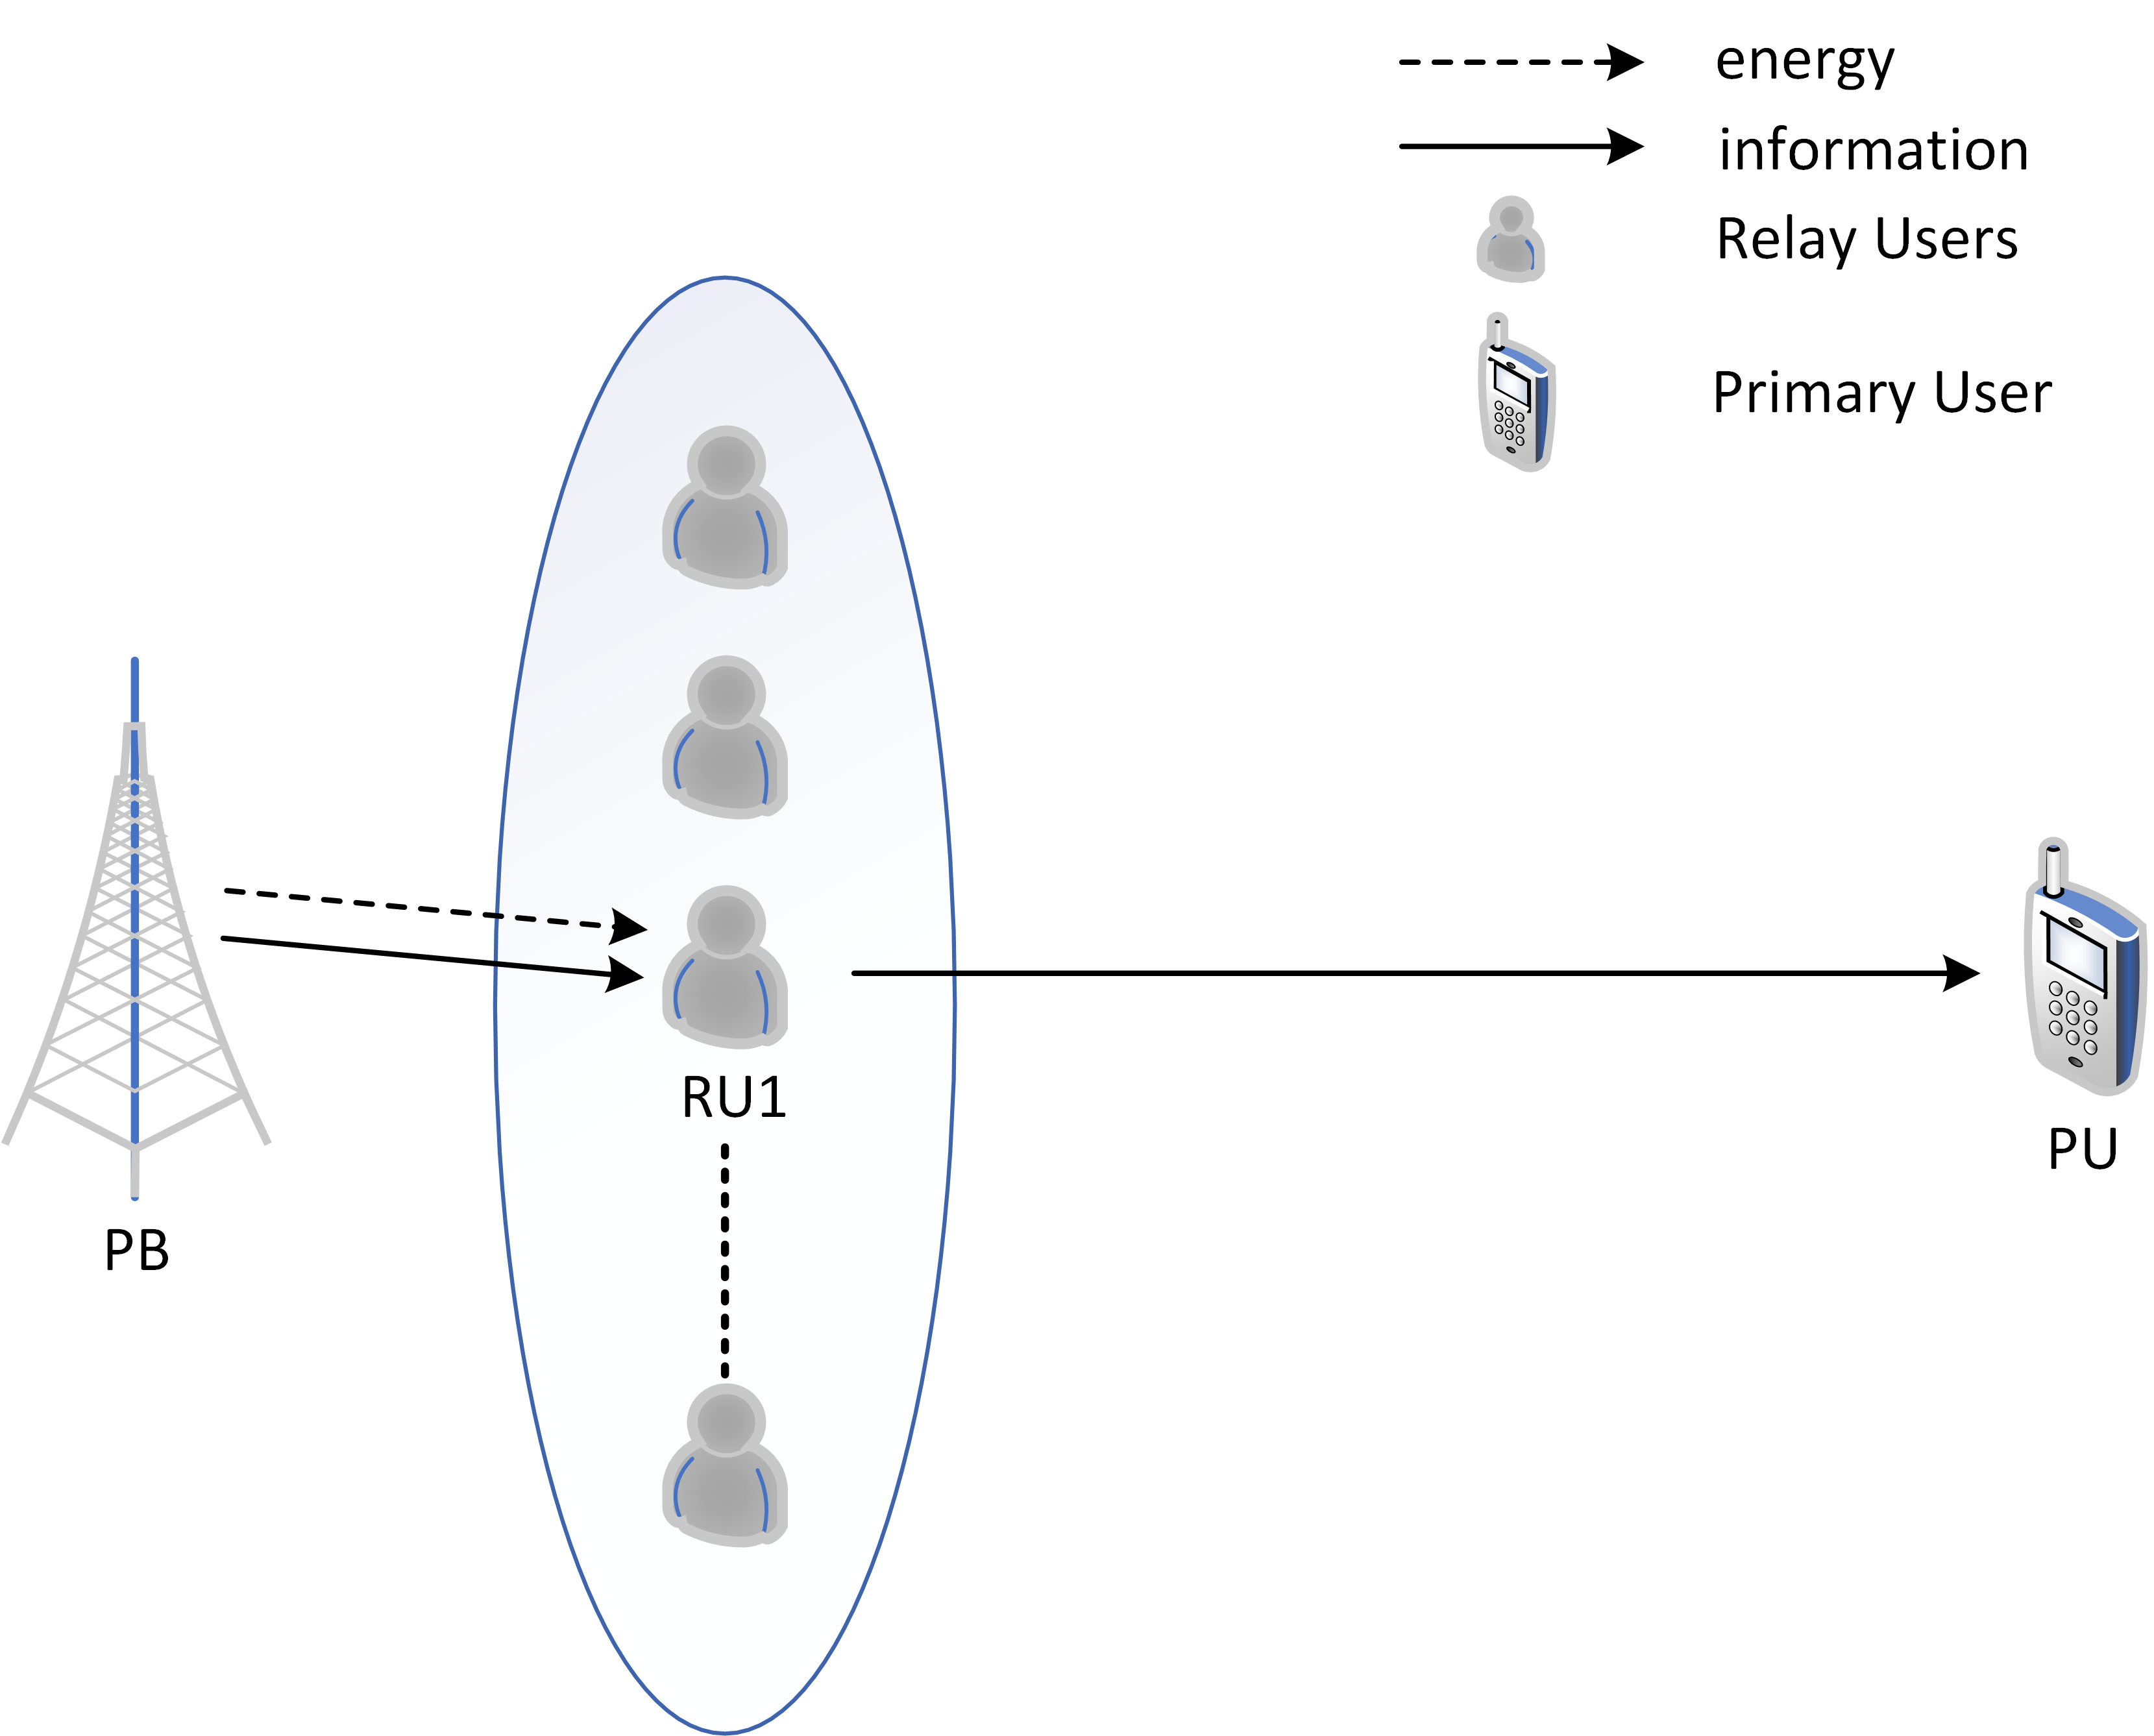
\includegraphics[width=8cm,keepaspectratio]{1.png}}
\caption{The system model.}
\label{fig}
\end{figure}

Since only a single link is considered, that is, the relay user obtains the transmitted data from the base station and extends the life of the communication network by obtaining energy from the RF signal, then the target user receives the signal from the relay user. Specifically, this framework is divided into two stages, as shown in Figure Figure 2. The total transmission duration is in T. The PB transmits its information in the first stage, and the RU may collect the energy through its own EH circuit from the received signal, and the duration of the stage is $\tau$T. In this stage, the collection of energy and the reception of the signal are conducted in the form of power segmentation, that is, this part of $\rho$ is used for the reception of the signal, and this part of 1-$\rho$ is used for the energy collection, where $\tau$ and $\rho$ are the two ratio coefficients in the interval (0,1). Assuming that the distance between the PB and the PU is greater than the transmission limit, this means that the PU cannot correctly receive the information from the PB in the first stage. In the second phase, the RU transmits the information received in the first phase to the PU, where the duration of the second stage is (1-$\tau$)T.

%\renewcommand{\arraystretch}{1.5}
%\newcolumntype{F}{>{$}c<{$}}
%\begin{table}[]
%\begin{tabular}{|c|c|}
%\hline
%PT to SU (SWIPT) & SU to PR (WIT)       \\ \hline
%1-$\rho$ (EH)    & \multirow{2}{*}{ID} \\ \cline{1-1}
%$\rho$ (ID)      &                     \\ \hline
%\end{tabular}
%\end{table}

\begin{figure}[htbp]
\centerline{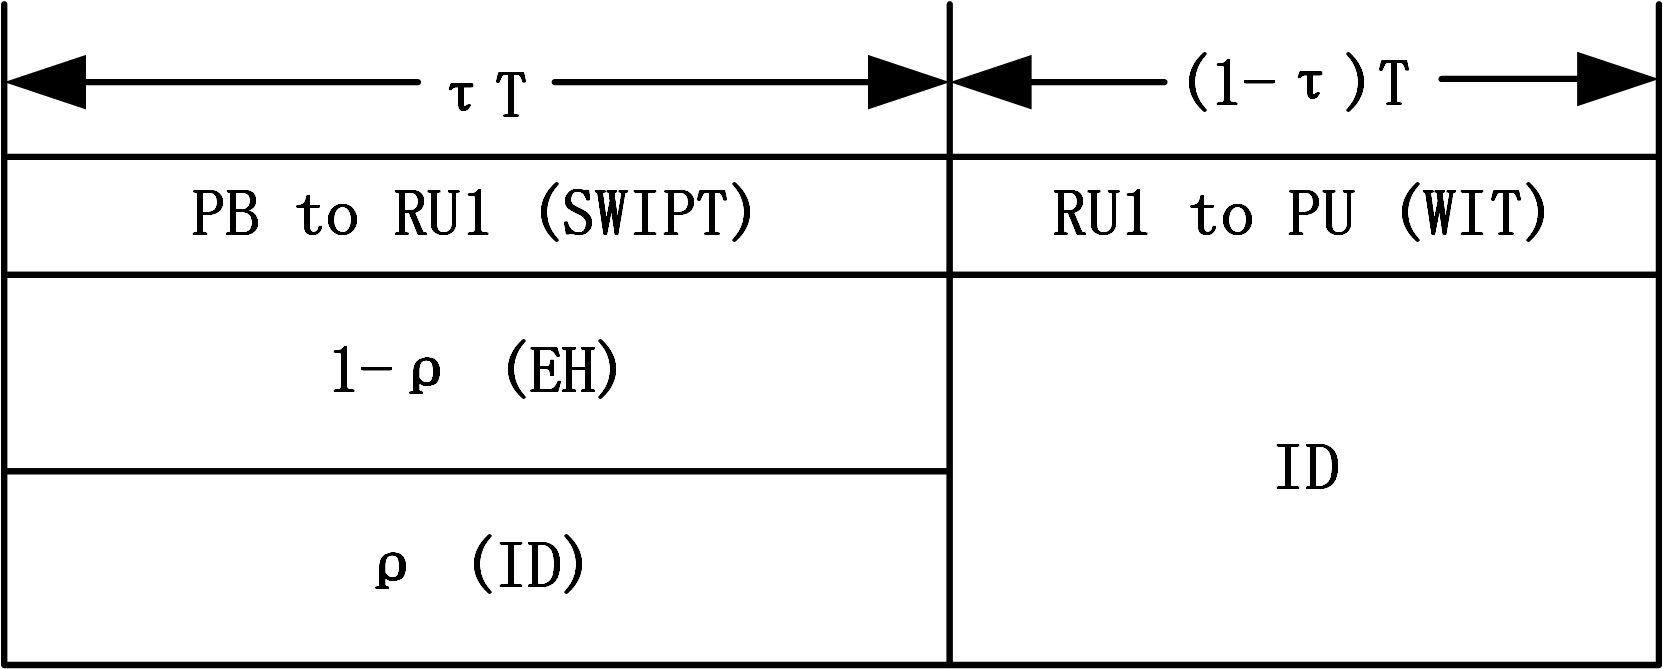
\includegraphics[width=7cm,keepaspectratio]{2.png}}
\caption{ The time division.}
\label{fig}
\end{figure}

\begin{figure}[htbp]
\centerline{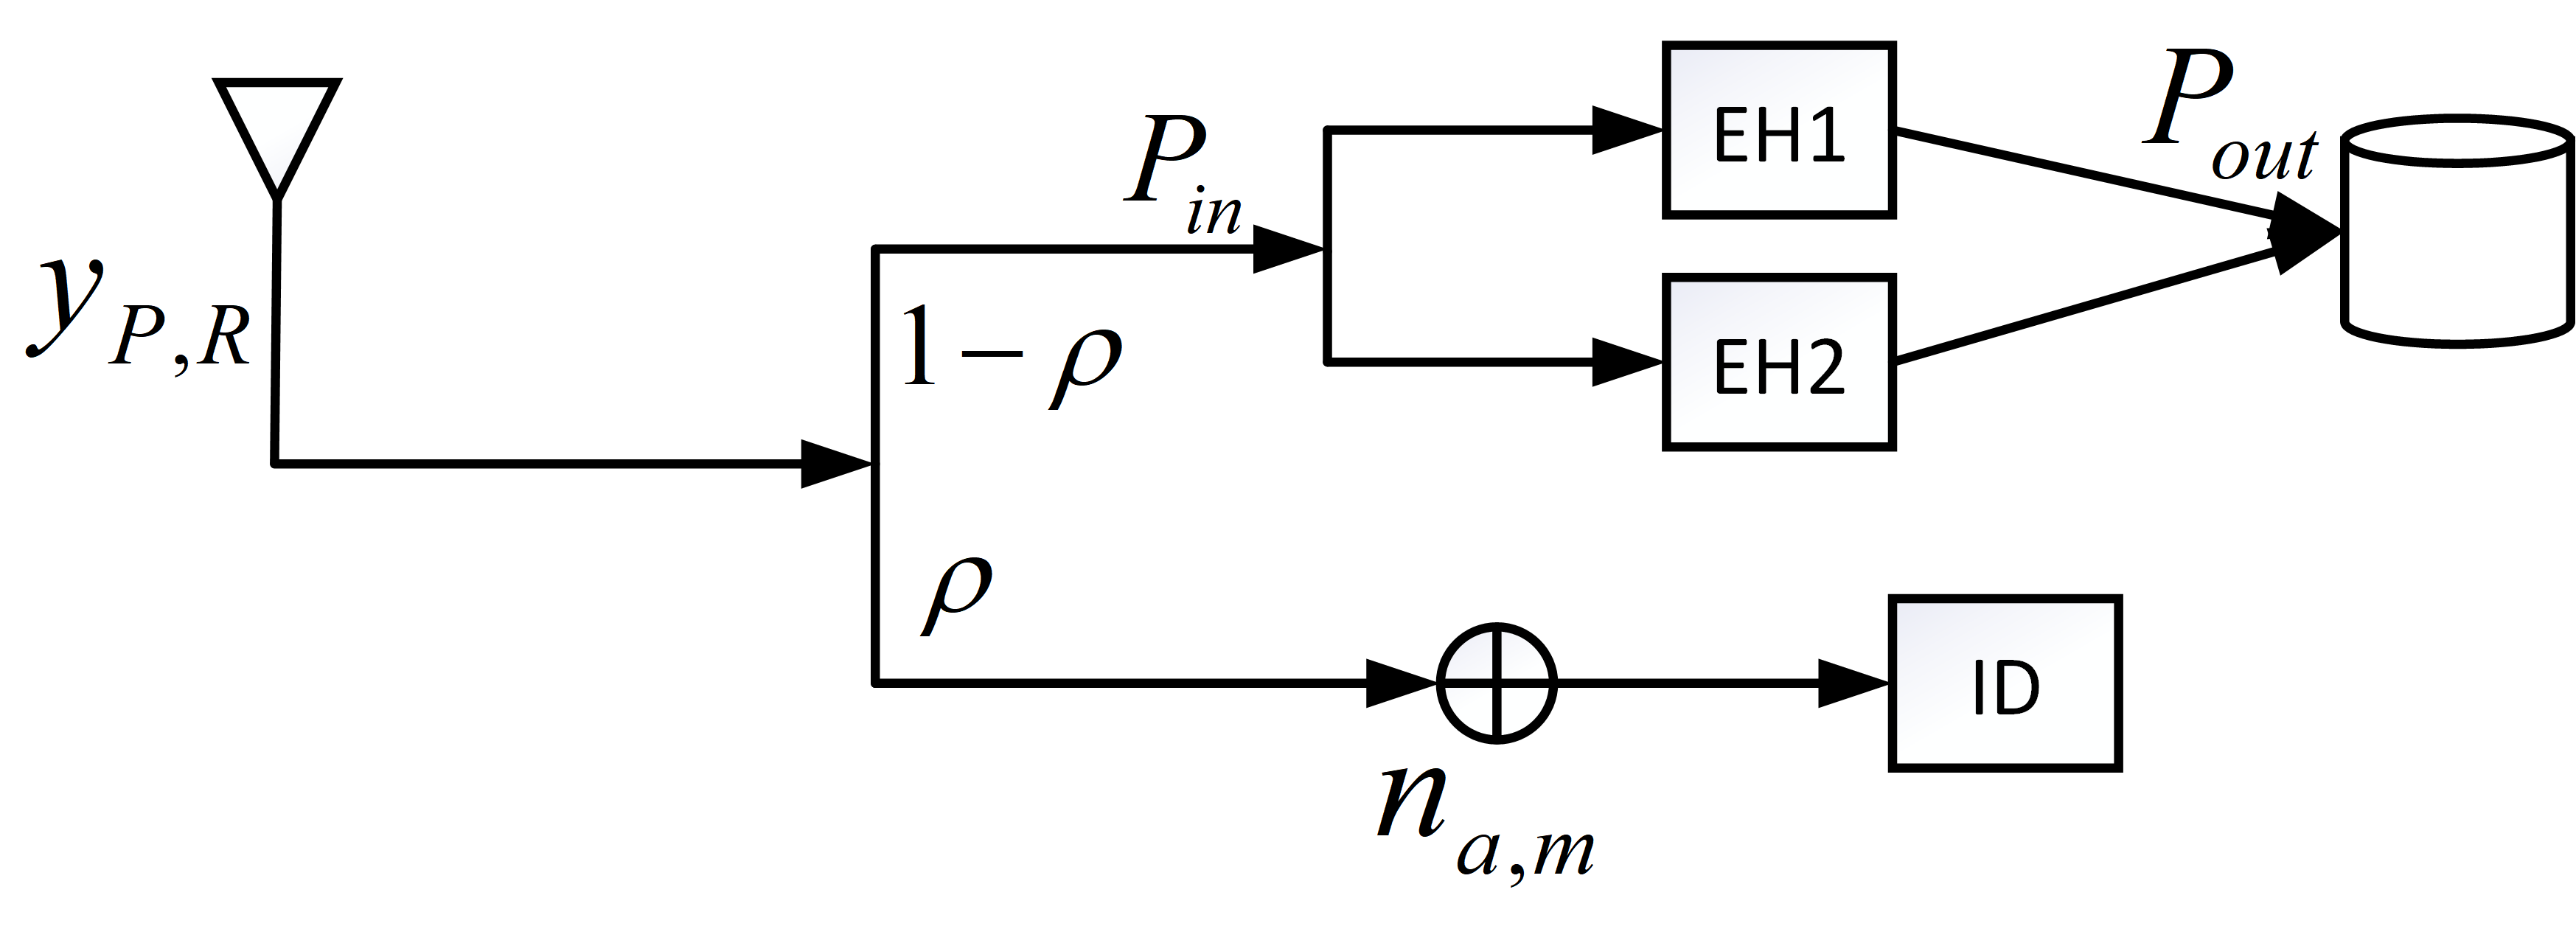
\includegraphics[width=8cm,keepaspectratio]{3.png}}
\caption{ A Schematic of the relay user.}
\label{fig}
\end{figure}


\subsection{Channel Model and Information Transmission}\label{BB}

Block flat fading channel is assumed, so the channel vectors remain constant within a block. The channel is modeled as
\begin{equation}\label{eqn-1} 
h= \beta d^{-m}
\end{equation}
where $\beta$ is the fixed loss, d is the distance between the transmitter and the receiver, and m is the path fading index.In each time slot, the transmit signal at the transmitter consists the information signals for authorized receivers, which is given by
\begin{equation}\label{eqn-1} 
x=ws
\end{equation}
where $s\in CN\left ( 0,1 \right )$ denotes the information symbol at the transmitting antenna, and without loss of generality, it is assumed that $E\left \{ \left |s  \right |^{2}   \right \} = 1$. $w\in C^{N\times 1}$ is the beamforming vector associated with the  relay user. 

For the relay user, the received signal is
\begin{equation}\label{eqn-1} 
y_{P,R} =h_{P,R}^{H} \cdot x
\end{equation}
The signal part for information transmission is
\begin{equation}\label{eqn-1}
y_{P,R}^{(ID)} = \sqrt{\rho }\cdot y_{P,R}+  n_{a,m}= \sqrt{\rho }h_{P,R}^{H}ws+  \delta _{a,m}^{2}
\end{equation}
where $n_{a,m}\sim CN\left ( 0,\delta _{a,m}^{2}   \right )$ is the additive white Gaussian noises (AWGN) at the relay user with $\delta _{a,m}^{2} $ denoting the noise power. 
The signal part for EH is
\begin{equation}\label{eqn-1}
y_{P,R}^{(EH)} = \sqrt{1-\rho }\cdot y_{P,R} = \sqrt{1-\rho }h_{P,R}^{H}ws
\end{equation}
Following (5), the input power before the relay user reaches the EH circuit is 
\begin{equation}\label{eqn-1}
P_{in} = \left ( 1-\rho  \right ) \left | h_{P,R}^{H}w  \right | ^{2}
\end{equation}

\subsection{Non-Linear EH Model}\label{BB}

If the ordinary linear EH model is used, then the output power through the EH circuit is proportional to the previous input power. Although the model is simple, it does not conform to the actual EH circuit. Due to various nonlinear electronic components, such as diodes, the RF-DC conversion efficiency depends on the input RF power level. This indirectly leads to the nonlinear characteristics of EH circuit. As shown in Fig.4, unlike the traditional linear EH model, the output DC power of the diode model cannot exceed the limit of the maximum output DC power due to its reverse breakdown voltage. It can be seen that the linear EH model is very different from the actual nonlinear EH model. Therefore, if the linear EH model is used in the system design, the mismatch caused by the linear EH model cannot be ignored. Therefore, this paper adopts the nonlinear EH model.

\begin{figure}[htbp]
\centerline{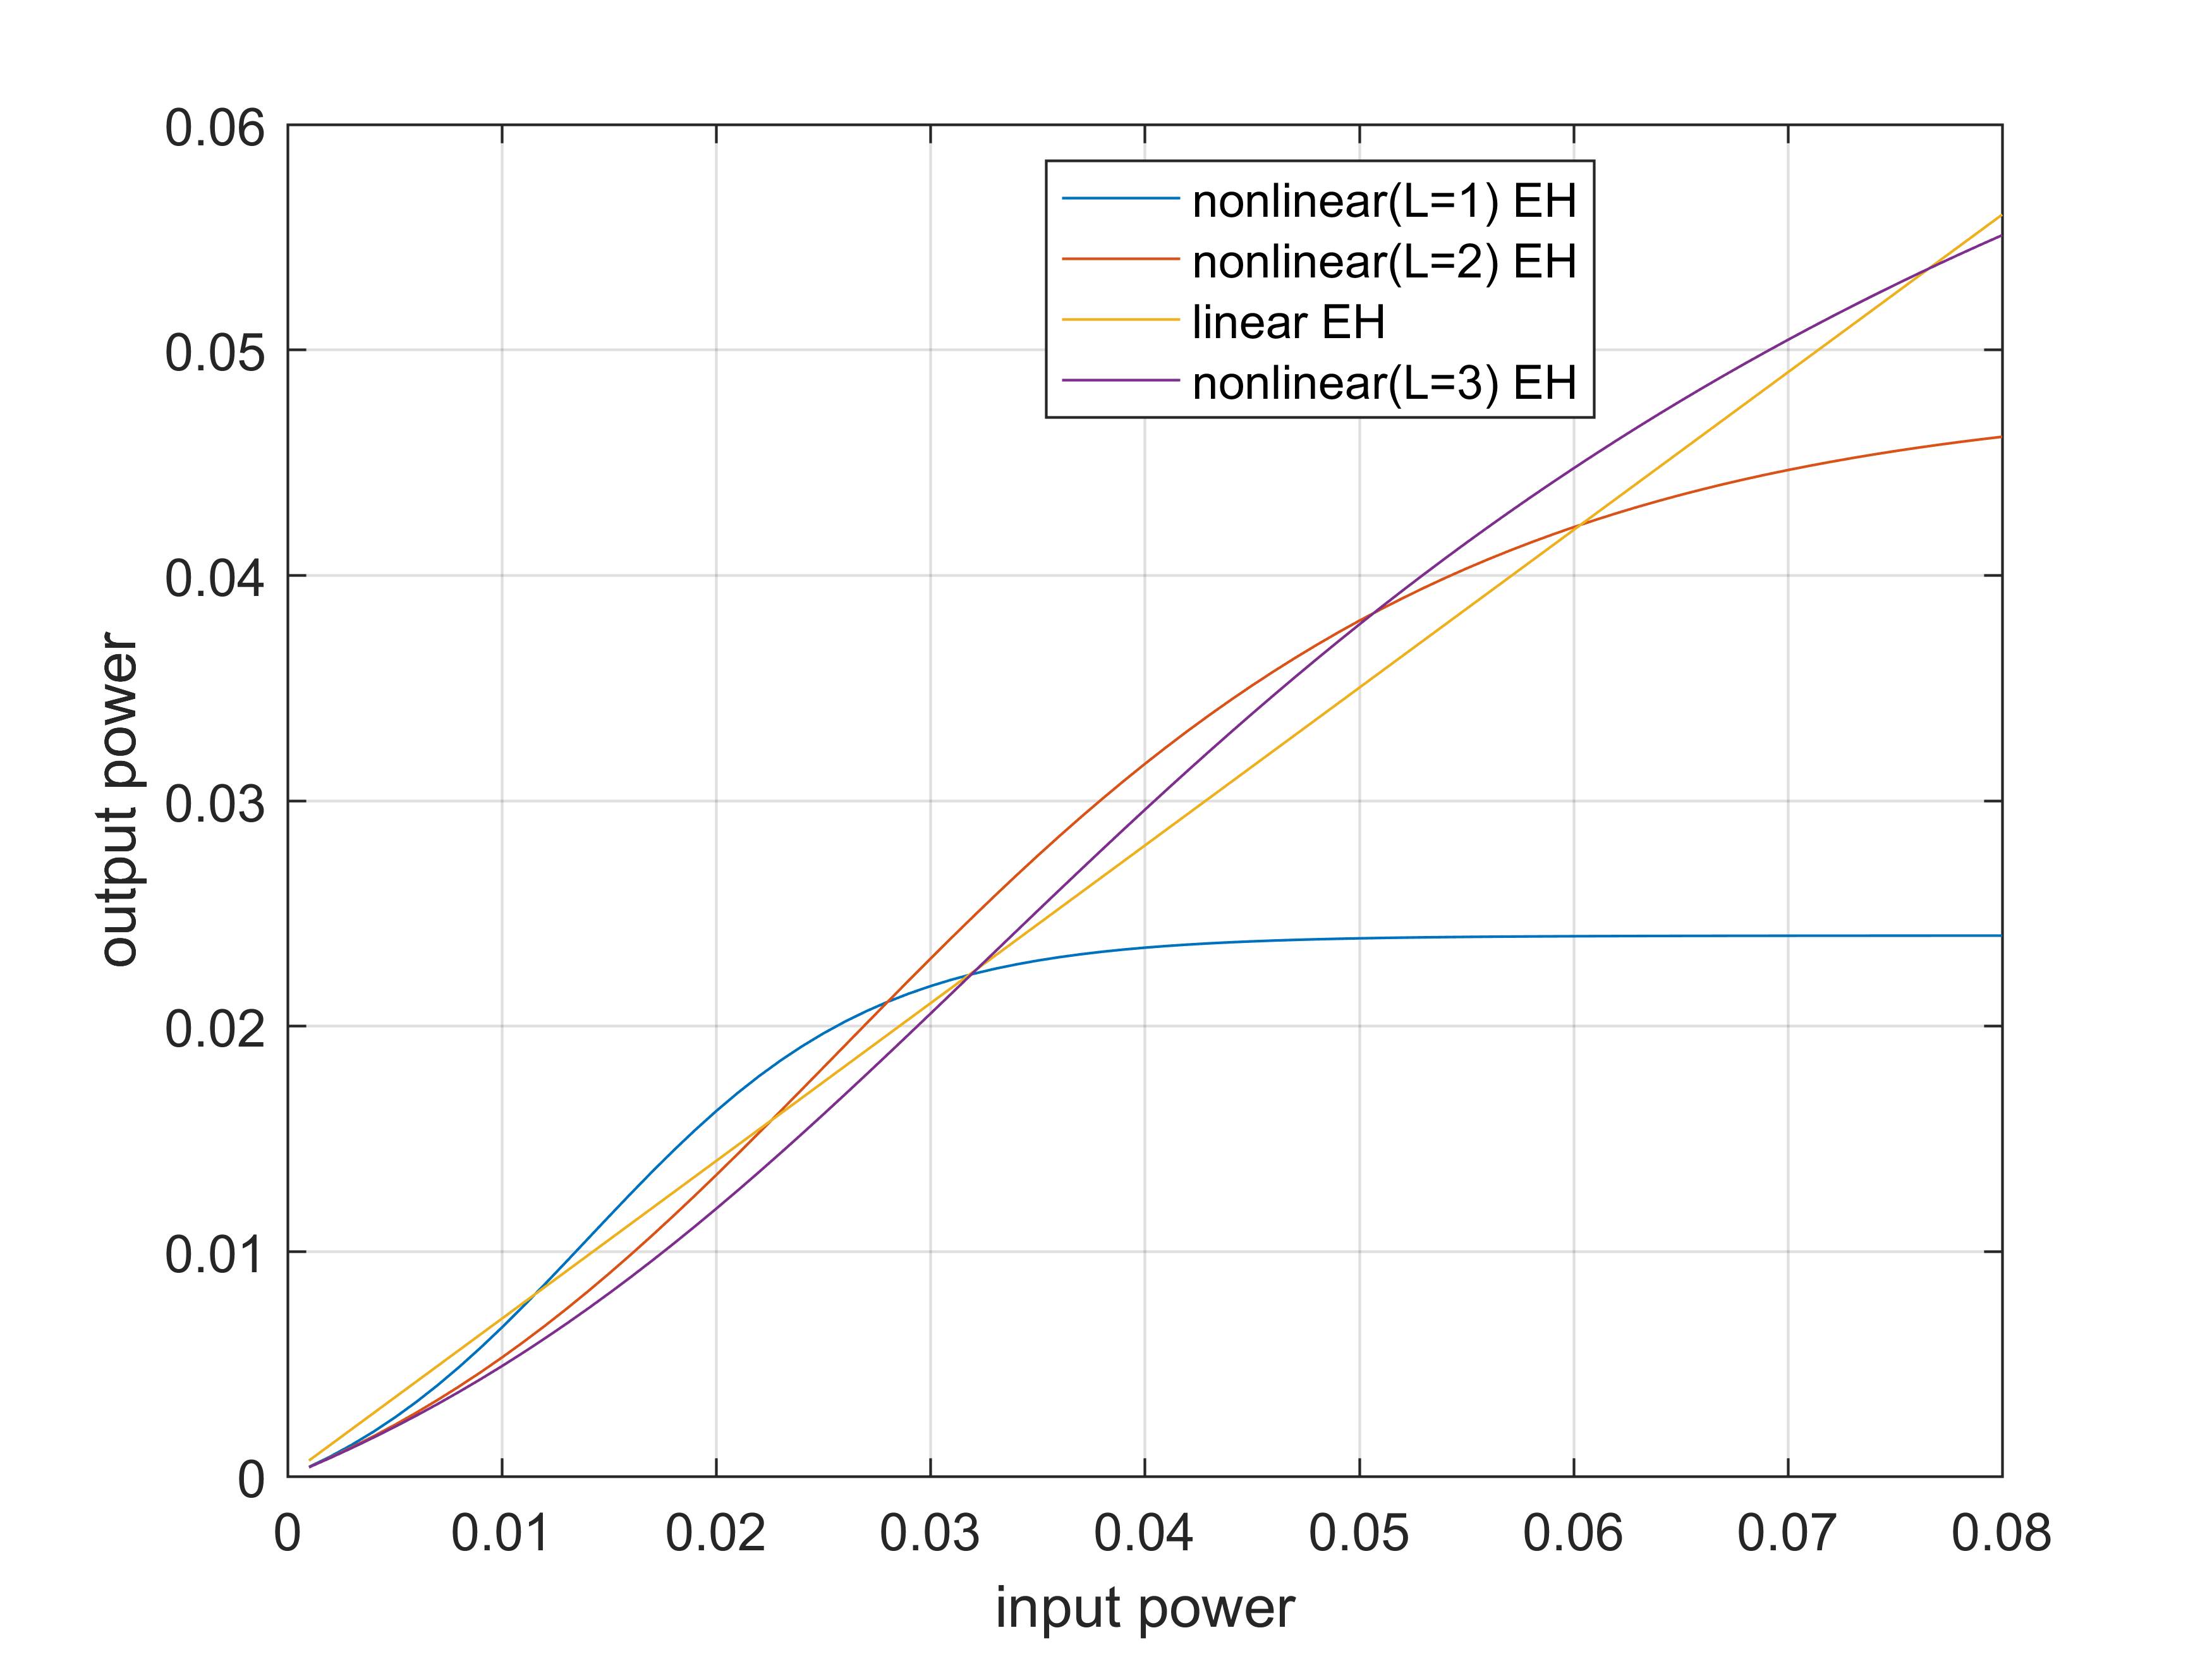
\includegraphics[width=9cm,keepaspectratio]{4.png}}
\caption{ Under the linear EH model and the nonlinear EH model, the harvested power and the input RF power are obtained.}
\label{fig}
\end{figure}

In Fig.4, we can also observe that the nonlinear EH model has lower RF-DC conversion efficiency than the linear EH model when the input RF power is very low. However, as the input RF power increases, the RF-DC conversion efficiency of the nonlinear EH model gradually increases and begins to outperform the linear model. However, due to the existence of nonlinear electronic devices, the parameters of the circuit will limit the output DC power, which will lead to the output power can not be infinitely increased, which will lead to the conversion efficiency of the nonlinear EH circuit is reduced. Obviously, increasing the number of EH circuits will increase the threshold of output RF power. This is because l-EH circuits divide the received RF signal into L streams, each stream is input into an EH circuit, and the power of each stream is guaranteed to be less than the total power. This method can avoid the EH circuit working in the saturation region and indirectly improve the RF-DC conversion efficiency of the EH circuit. 
It should be noted that the number of circuits cannot be infinitely increased, because the superposition of EH circuits will increase the circuit loss and reduce the RF-DC conversion efficiency in a certain input RF power range.

Let $\alpha _{l} $ be the weight of the l-th EH circuit, it must satisfy
\begin{equation}\label{eqn-1}
{\textstyle \sum_{l=1}^{L}} \alpha _{l} = 1
\end{equation}

The output power obtained by this EH architecture is 
\begin{equation}\label{eqn-2}
  \begin{aligned}
	P_{out}^{} &= {\textstyle \sum_{l=1}^{L}} \left [ \frac{\frac{M}{1+e^{\left [ -a\left ( \alpha _{l} P_{in}-b  \right )  			\right ] } }- \frac{M}{1+e^{ab} }  }{1-\frac{1}{1+e^{ab} } }  \right ] \\ 
	&= {\textstyle \sum_{l=1}^{L}} \left [ \frac{M}{X\left ( 1+e^{\left [ -a\left ( \alpha _{l}  P_{in} -b\right )  \right ] }  	\right ) } -Y \right ]
  \end{aligned}
\end{equation}
where $X= \frac{e^{ab} }{1+e^{ab} }$ , $Y= \frac{M }{e^{ab} }$. $M$,$a$,$b$ are constants, $M$ denotes the maximum limitation on output DC power while$a$and$b$represent the resistance, the capacitance and the circuit sensitivity. It is noticed that traditional EH receiver architecture with single EH circuit can be regarded as a special case of our proposed PTS EH receiver architecture by inputing all received RF signals into one EH circuit.

\subsection{Problem Formulation}\label{BB}

Considering long-distance communication, RU as a relay user, we can ensure the stability of this communication link from two aspects. On the one hand, it is the causal relationship of data transmission. It is necessary to ensure that the output signal from the base station can be received by the relay user and has sufficient energy to support the relay user to send the signal to the target user. On the other hand, there is a causal relationship between energy collection and consumption. In order to prolong the service life, it is necessary to make the energy collected by the relay user from the RF signal in the first stage greater than the energy consumed by itself in the second stage. This is not only the condition for the stability of this communication link, but also the essence of SWIPT.

The energy causality satisfying the current communication link is that the energy received by the relay user in the first stage is greater than the energy consumed by the relay user as the signal sender in the second stage. That is to say 
\begin{equation}\label{eqn-1}
E_{harvest}=P_{out}\cdot \tau T\ge E
\end{equation}
where $E$ is the energy consumed in the second stage. In particular, when the energy harvested in the first stage is used for the consumption of the transmitted signal in the second stage, that is, when $E_{harvest}= E$, the efficiency is the highest and the performance of the system is the best. Therefore, the SNR of the second stage can be expressed by 
\begin{equation}\label{eqn-1}
SNR_{R,P}  =\frac{P_{out}\cdot \tau T\cdot h_{R,P}  }{\left ( 1-\tau   \right ) \cdot T\cdot \sigma _{b,m}^{2}}
\end{equation}

The relay user will complete the transmission of information in the form of decoding and forwarding, so the throughput of the total data transmitted through PT is 
\begin{equation}\label{eqn-1}
\Omega = \min\left \{ \tau T\cdot R_{P,R} \ ,\ \left ( 1-\tau  \right )T\cdot R_{R,P} \right \}
\end{equation}
where $R_{P,R}$ and $R_{R,P}$ are the data transfer rates from PB to RU and from RU to PU, respectively.  Can be expressed as
\begin{equation}\label{eqn-1}
R_{P,R} = \log_{2}\left ( 1+\frac{\sqrt{\rho }\left |h_{P,R}^{H}w   \right |^{2}   }{\delta _{a,m}^{2} }  \right )
\end{equation}
\begin{equation}\label{eqn-1}
R_{R,P} = \log_{2}\left ( 1+\frac{P_{out}\cdot \tau T\cdot h_{R,P}  }{\left ( 1-\tau   \right ) \cdot T\cdot \sigma _{b,m}^{2}}  \right )
\end{equation}


This communication link attempts to consume the minimum energy while satisfying the two causality of data transmission and energy constraints. Therefore, the optimization problem of this communication network is formulated as 
\begin{equation*}
\begin{split}
P1:&\min_{\rho , \tau , w , \alpha_{l}} \,\, \tau T\cdot \left \| w \right \|^{2}\\
&s.t.\quad  \left\{\begin{array}{lc}
\left \| w \right \| ^{2} \le P_{max} \qquad \qquad \qquad \qquad \, \notag{C1}\\
\log_{2}\left ( 1+\frac{\sqrt{\rho }\left |h_{P,R}^{H}w   \right |^{2}   }{\delta _{a,m}^{2} }  \right )\ge R_{0} \ \ \quad \notag{C2}\\
\log_{2}\left ( 1+\frac{P_{out}\cdot \tau T\cdot h_{R,P}  }{\left ( 1-\tau   \right ) \cdot T\cdot \sigma _{b,m}^{2}}  \right ) \ge R_{1} \ \quad \notag{C3}\\
{\textstyle \sum_{l=1}^{L}}\alpha _{l}= 1,\forall \alpha _{l}\ge 0 \qquad \qquad \ \ \, \notag{C4}\\
\rho ,\tau \in \left ( 0,1 \right ) \qquad \qquad \qquad \qquad \ \ \notag{C5}\\
E_{harvest}= E \qquad \qquad \qquad \qquad \, \notag{C6}\\
\end{array}\right.
\end{split}
\end{equation*}

%$\qquad \qquad \qquad \qquad \qquad \quad \tau T\cdot R_{P,S} \ge A \qquad \quad \ \, \notag{C3}$

$C1$ is the base station transmit power constraint, $P_{max}$ is the total available power. 
$C2$ denotes the data transmission rate constraint of SWIPT from base station to relay user in the first stage. 
$C3$ represents the data transmission rate constraint of the target user in the second stage.
%$C4$ represents the data throughput constraint of this communication link, where $A$ represents the required threshold of PT data throughput. 
$C4$ is the weight constraint of each EH circuit. 
$C5$ is the constraint of power splitting ratio and time splitting ratio.
$C6$ is  the energy constraint collected by the relay user in the first stage.

It can be seen that the optimization problem contains nonlinear constraints, and there is a coupling of multiple variables, which cannot be solved by traditional methods. Therefore, we design an effective solution for it in Section IV.

\section{Solution Approach}
Problem P1 is solved with the following idea. Firstly, we optimize the weight $\alpha _{l}$ of the proposed multi-EH circuit. Considering that too many EH circuits will increase the corresponding circuit loss and reduce the conversion efficiency, only two EH circuits are considered in this communication link. Moreover, the optimization of $\alpha _{l}$ is independent of the optimization of $\left \{ \rho ,\tau ,w \right \}$. This is because after giving the EH architecture of the relay user, the original optimization problem has a corresponding suboptimal solution, and then compares the suboptimal solutions under different weight ratios. The result is the minimum energy consumption of the base station. Therefore, we can use the optimization of $\alpha _{l}$ as the outermost layer and the optimization of $\left \{ \rho ,\tau ,w \right \}$ as the inner layer to solve P1. For the optimization of $\left \{ \rho ,\tau ,w \right \}$ in the inner layer, due to the coupling of variables, we can first fix $\left \{ \rho ,w \right \}$, find the optimal solution of $\tau$, and then fix $\tau$, find the optimal solution of $\left \{ \rho ,w \right \}$, so as to solve the optimal value by alternating iteration, in which CVX can be used to assist the solution.

\subsection{Optimization of $\left \{ \rho,\tau,w \right \}$}\label{BB}
The optimization of the inner variables requires the use of alternating iterative optimization, in which the CVX solver is nested.

Firstly, fixed $\left \{ \rho ,w \right \}$, the optimal solution of $\tau$ is solved. It can be achieved by solving the problem P2.
$$P2:\underset{\tau}{\min} \ \tau T\cdot \left \| w \right \|^{2}$$
$\qquad \qquad \qquad \qquad \qquad  s.t.\ \ \notag{C3},  \notag{C5},  \notag{C6}$

Since $\left \{ \rho ,w \right \}$ is fixed, the problem P2 can be simplified into a linear optimization problem by dealing with constraints. Therefore, C3 can be represented by 
\begin{equation}\label{eqn-1}
\tau \ge1- \frac{P_{out} \cdot h_{R,P} }{\left ( 2^{R_{1} }-1  \right )\sigma _{b,m}^{2}+P_{out} \cdot h_{R,P}  }
\end{equation}  
The objective function in P2 is a linear function of $\tau$, and decreases with the decrease of $\tau$, so the optimal value $\tau ^{\ast }$ is obtained at the boundary.

Then the optimal solution $\tau ^{\ast }$ of the above optimization problem is fixed as a known quantity, and then the optimal solution of $\left \{ \rho ,w \right \}$ can be solved by problem P3. However, due to the nonlinearity of the EH circuit electronic device, the output power has a threshold, that is, the output RF power of the EH circuit will not increase indefinitely with the increase of the input RF power, so the problem P3 is nonlinear and needs to be further transformed. 
In this paper, variable substitution and inverse function are used to deal with nonlinear constraints and the input RF power is used instead of the output to convert it into a linear constraint. so that the problem P3 is solved to the optimal values $\left \{ \rho^{\ast } ,w^{\ast } \right \}$.
$$P3:\underset{\rho,w}{\min} \ \tau T\cdot \left \| w \right \|^{2}$$
$\qquad \qquad \qquad \qquad   s.t.\ \ \notag{C1}, \notag{C2}, \notag{C3}, \notag{C4}, \notag{C5}, \notag{C6}$

By defining $W= ww^{H}$, The total power constraint can be expressed as $Tr\left ( W \right )\le P_{max}$, By converting the quadratic form into a linear form, reduce the computational complexity. The communication rate of relay users can be represented by 
\begin{equation}\label{eqn-1}
R_{P,R} = \log_{2}\left ( 1+\frac{\sqrt{\rho }\cdot h_{P,R}^{H}Wh_{P,R}     }{\delta _{a,m}^{2} }  \right )
\end{equation} 
The communication rate constraint of the relay user can be expressed as 
\begin{equation}\label{eqn-1}
h_{P,R}^{H}Wh_{P,R} \ge \frac{\left ( 2^{R_{0} }-1  \right )\sigma _{a,m}^{2}  }{\sqrt{\rho } }
\end{equation} 
In the process of relay user to target user communication, due to the non-convex constraint of energy harvesting, it is solved by variable substitution and inverse function. The communication rate constraint of the target user can be expressed as
\begin{equation}\label{eqn-1}
P_{out(in)} \ge \frac{\left ( 2^{R_{1} }-1  \right )\left ( 1-\tau  \right ) \sigma _{b,m}^{2}  }{\tau \cdot h_{R,P} }
\end{equation}  
The input RF power of the EH circuit can be expressed as $P_{in} =  \left ( 1-\rho  \right )\left | h_{P,R}^{H}w  \right | ^{2} $. The inverse function of the input RF power with respect to the output RF power is $P_{in(P_{out} )} = {\textstyle \sum_{l=1}^{L}} P_{in(P_{out(l)} )}$, where 
\begin{equation}\label{eqn-1}
P_{in(P_{out(l)} )} =-\frac{1}{a\alpha _{l} }\ln \frac{e^{ab}(M-P_{out(l)}) }{e^{ab}P_{out(l)}+M} +\frac{b}{\alpha _{l} }
\end{equation}  
Inside this, $P_{out(l)}=x \alpha _{l}$, and $x=\frac{\left ( 2^{R_{1} }-1  \right )\left ( 1-\tau  \right ) \sigma _{b,m}^{2}  }{\tau \cdot h_{R,P} } $, $\alpha _{l}$ is the weight of each EH circuit. As mentioned above, the input RF power constraint can be used to replace the output radio frequency power constraint. Therefore $P_{in(P_{out} )} \le \left ( 1-\rho  \right )\left | h_{P,R}^{H}w  \right |^{2}$.

Since the problem P3 satisfies the Slater's condition, the strong duality is maintained, and the optimal power splitting ratio $\rho^{\ast}$ in P3 can be obtained by Lagrange dual decomposition. 
Firstly, the Lagrangian function of problem P3 is 
\begin{equation}\label{eqn-2}
  \begin{aligned}
	L(\rho ,\lambda )&=\tau T\cdot Trace(W) \\& +\lambda _{1} (  \frac{\left ( 2^{R_{0} }-1  \right )\sigma _{a,m}^{2}  }				{\sqrt{\rho } }-h_{P,R}^{H}Wh_{P,R}) \\& +\lambda _{2}(P_{in(P_{out} )} - \left ( 1-\rho  \right )h_{P,R}^{H}Wh_{P,R}) 
  \end{aligned}
\end{equation}
where $\lambda=[\lambda_{1} , \lambda_{2}]$ is the Lagrangian multiplier and $\lambda_{1} , \lambda_{2}\ge 0$. 
Then we can get the dual function of (19) is 
\begin{equation}\label{eqn-2}
  \begin{aligned}
	D(\lambda )=\underset{\rho}{\min} \ L(\rho,\lambda )
  \end{aligned}
\end{equation}

The dual problem is expressed as
$$P4:\underset{\lambda}{\min} \ D(\lambda )$$
$\qquad \qquad \qquad  \qquad \quad  s.t.\ \ \lambda_{1} , \lambda_{2}\ge 0$

The optimal solution of problem P4 can be determined by gradient projection method. First, the subgradient of $\lambda$ is
\begin{equation}
\left\{
\begin{aligned}
%\nonumber
&S_{\lambda _{1} } =\frac{\left ( 2^{R_{0} }-1  \right )\sigma _{a,m}^{2}  }{\sqrt{\rho } }-h_{P,R}^{H}Wh_{P,R}\\
&S_{\lambda _{2} } =P_{in(P_{out} )} - \left ( 1-\rho  \right )h_{P,R}^{H}Wh_{P,R}\\
\end{aligned}
\right.
\end{equation}

In each iteration, the Lagrangian multiplier $\lambda$ is updated to
\begin{equation}
\left\{
\begin{aligned}
%\nonumber
&\lambda _{1}(z+1)=[\lambda _{1}(z)+\delta _{1} S_{\lambda _{1}} ]^{+} \\
&\lambda _{2}(z+1)=[\lambda _{2}(z)+\delta _{2} S_{\lambda _{2}} ]^{+} \\
\end{aligned}
\right.
\end{equation}
where $[\cdot ]^{+} =$ max$\left \{ 0,\cdot  \right \}  $, and $\delta _{1} ,\delta _{2} $ denote the iterative step size, which are positive.


Therefore, the optimal power splitting ratio can be calculated by applying the KKT condition, which are given as

\begin{equation}
\left\{
\begin{aligned}
%\nonumber
&\frac{\partial L(\rho ,\lambda )}{\partial \rho } = 0\\
&\lambda _{1} (  \frac{\left ( 2^{R_{0} }-1  \right )\sigma _{a,m}^{2}  }{\sqrt{\rho } }-h_{P,R}^{H}Wh_{P,R}) = 0\\
&\lambda _{2}(P_{in(P_{out} )} - \left ( 1-\rho  \right )h_{P,R}^{H}Wh_{P,R}) = 0\\
\end{aligned}
\right.
\end{equation}
Based on the (23), $\rho ^{\ast }$ can be expressed as 
\begin{equation}\label{eqn-1}
\rho ^{\ast }=(\frac{\lambda _{1}(2^{R_{0}-1 }\sigma _{a,m}^{2}  ) }{\lambda _{2}h_{P,R}^{H}Wh_{P,R}} )^{\frac{2}{3} }
\end{equation} 
Then the feasible solution of $W_{(z)}$ can be solved by cvx, and iterates with $\rho _{(z)}$ and $\tau _{(z)}$ alternately. After reaching the convergence condition, it returns to its respective optimal solution. The specific algorithm is as follows: 
\begin{algorithm}
	%\textsl{}\setstretch{1.8}
	\renewcommand{\algorithmicrequire}{\textbf{Input:}}
	\renewcommand{\algorithmicensure}{\textbf{Output:}}
	\caption{Alternating Iterative Algorithm}
	\label{alg1}
	\begin{algorithmic}[1]
		\STATE Initialization: Primal variables $\rho _{(0)} ,\tau _{(0)} , w _{(0)},W _{(0)}$ , Lagrangian multiplier $\lambda _{1}^{(0)}  ,\lambda _{2}^{(0)}$ $ , z \leftarrow 0$
		
		\REPEAT
		\STATE Obtain $ \tau _{(z+1)}^{\prime }  $ by solving the problem P2
		\STATE Update $ \tau _{(z+1)} = \tau _{(z+1)}^{\prime }$ , fixation it and bring it as a known quantity
		\STATE Computes $\rho _{(z+1)}^{\prime } , W_{(z+1)}^{\prime }$ by solving the problem P3 and according to (23)
		\STATE Update $ \rho _{(z+1)} = \rho _{(z+1)}^{\prime } , W_{(z+1)} = W_{(z+1)}^{\prime }$
		\STATE $z \leftarrow z + 1$
		\UNTIL The iteration converges.
		\STATE   Set $  \rho ^{\ast } =\rho _{(z+1)}  , \tau ^{\ast } =\tau _{(z+1)} , W ^{\ast } =W _{(z+1)}   $
		\ENSURE  $(\rho ^{\ast } ,\tau ^{\ast } , W ^{\ast })$
	\end{algorithmic}  
\end{algorithm}

After obtaining the optimal value of $W$, the beamforming vector $w ^{\ast }$ can be obtained by the maximum rank decomposition.

\subsection{Optimization of $\alpha _{l}$ }\label{BB}

$\alpha _{l}$  is the proportion weight of each EH circuit, after it is fixed, each $\alpha _{l}  ^{\ast }$ will generate an optimal value of the corresponding problem P1, and the corresponding optimal solution $( {\rho^{\ast }} , {\tau^{\ast }} , {W^{\ast }} )$ is the optimal solution in the current $\alpha _{l}$ case. Our ultimate goal is to get the minimum energy consumption of the base station. Therefore, in the outer layer, the dichotomy of Algorithm 2 can be used to find the minimum energy consumption of the base station., the corresponding optimal solution is $\alpha _{l}  ^{\ast }$.

\begin{algorithm}
	%\textsl{}\setstretch{1.8}
	\renewcommand{\algorithmicrequire}{\textbf{Input:}}
	\renewcommand{\algorithmicensure}{\textbf{Output:}}
	\caption{Outer Optimization Algorithm}
	\label{alg1}
	\begin{algorithmic}[1]
		\STATE Initialization: $p\le \alpha _{l} \le q$
		
		\REPEAT
           \STATE Update $\alpha _{l}= (p+q)/2$
		\STATE Initialize $E_{out}^{(0)} $ , $P_{in}^{(0)}$ , and set $z=1$
		\STATE Obtain $\left \{ \rho _{(z)}^{\ast } ,\tau _{(z)}^{\ast },W _{(z)}^{\ast } \right \} $ by solving the problem P2 and P3
		\STATE Update $ E_{out}^{(z)}=E_{out}^{(z)\ast}$ , $z=z+1$
		\STATE if $E_{out}^{(z)}\le  E_{out}^{(z-1)}$ , update $q= \alpha _{l}$ ; else update $p= \alpha _{l}$
		\UNTIL $q-p< \varepsilon$
		\STATE   Set $\alpha _{l}^{\ast } = \alpha _{l} ,  E_{out}^{\ast} = E_{out}^{(z)}  $
		\ENSURE  $\alpha _{l}^{\ast }  , E_{out}^{\ast}$
	\end{algorithmic}  
\end{algorithm}

\subsection{Relay selection}\label{BB}

In the established optimization problem of minimizing the energy consumption of the base station, The communication rate of the two stages can be guaranteed under the constraint conditions, and the default is that there is no interruption problem. 
Due to the difference in the location of the relay user, the channel state information is different. In addition, the difference in the hardware facilities of the relay user will also lead to the difference in the fitted nonlinear energy harvesting curve. Therefore, for different relays, the energy consumption of the base station under the optimal time factor, power factor and weight ratio of EH circuit is considered respectively. This can be reflected in the simulation results, and the user with the lowest energy consumption of the base station is selected as the optimal relay user.



\section{Numerical Results}

This section provides some simulation results to discuss the system performance of nonlinear SWIPT relay cooperative communication. For the nonlinear EH model parameters, assume that $M=0.024$ corresponds to the threshold when the single EH circuit reaches saturation, and $a=150$ and $b=0.014$ are other circuit parameters. In addition, we simulate the RF conversion efficiency of the linear EH model to be $\eta=0.7$.



\begin{figure}[htbp]
\centerline{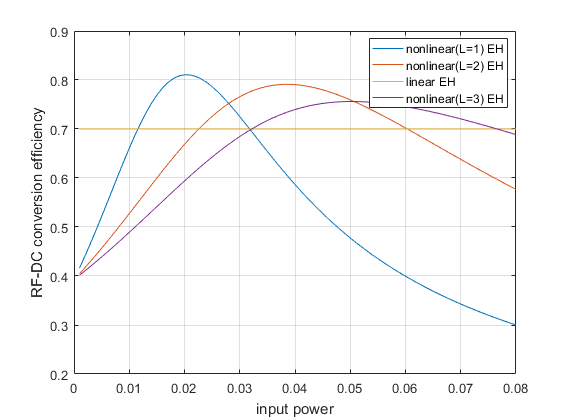
\includegraphics[width=9cm,keepaspectratio]{5.png}}
\caption{ Under linear EH model and nonlinear EH model, conversion efficiency and input RF power are obtained.}
\label{fig}
\end{figure}

\begin{figure}[htbp]
\centerline{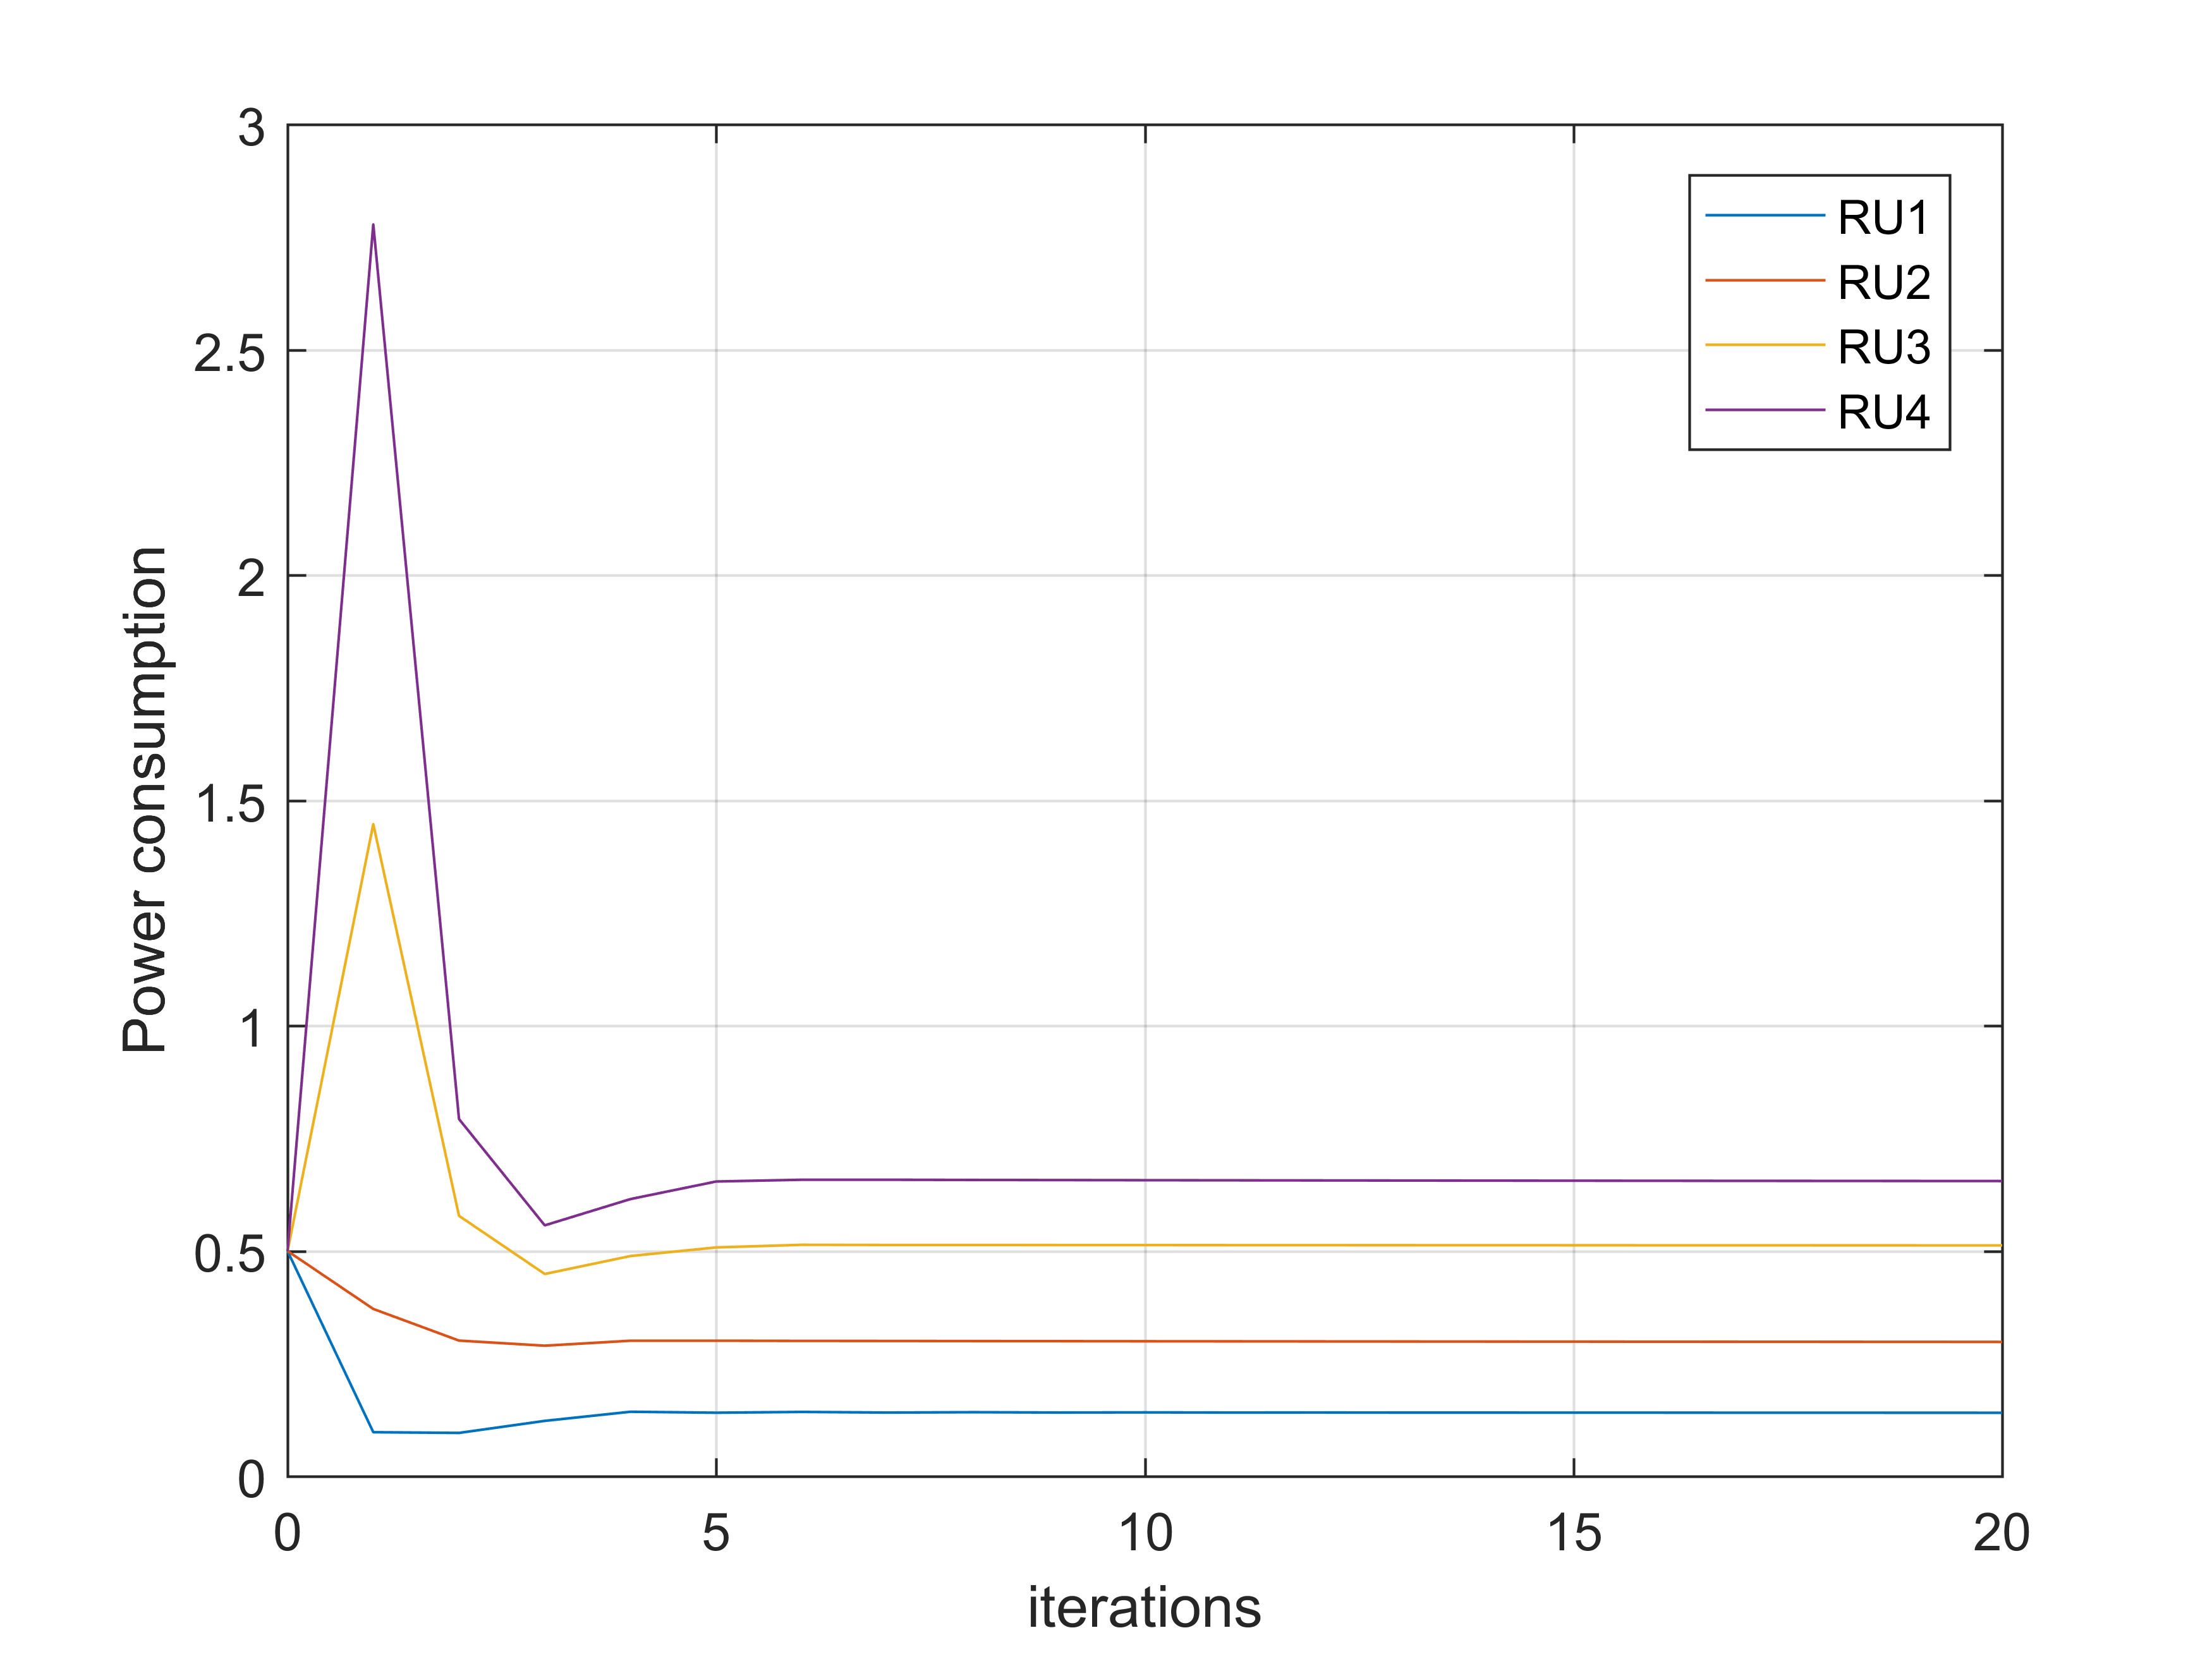
\includegraphics[width=9cm,keepaspectratio]{power consumption.png}}
\caption{ Base station energy consumption under different relay users.}
\label{fig}
\end{figure}

\begin{figure}[htbp]
\centerline{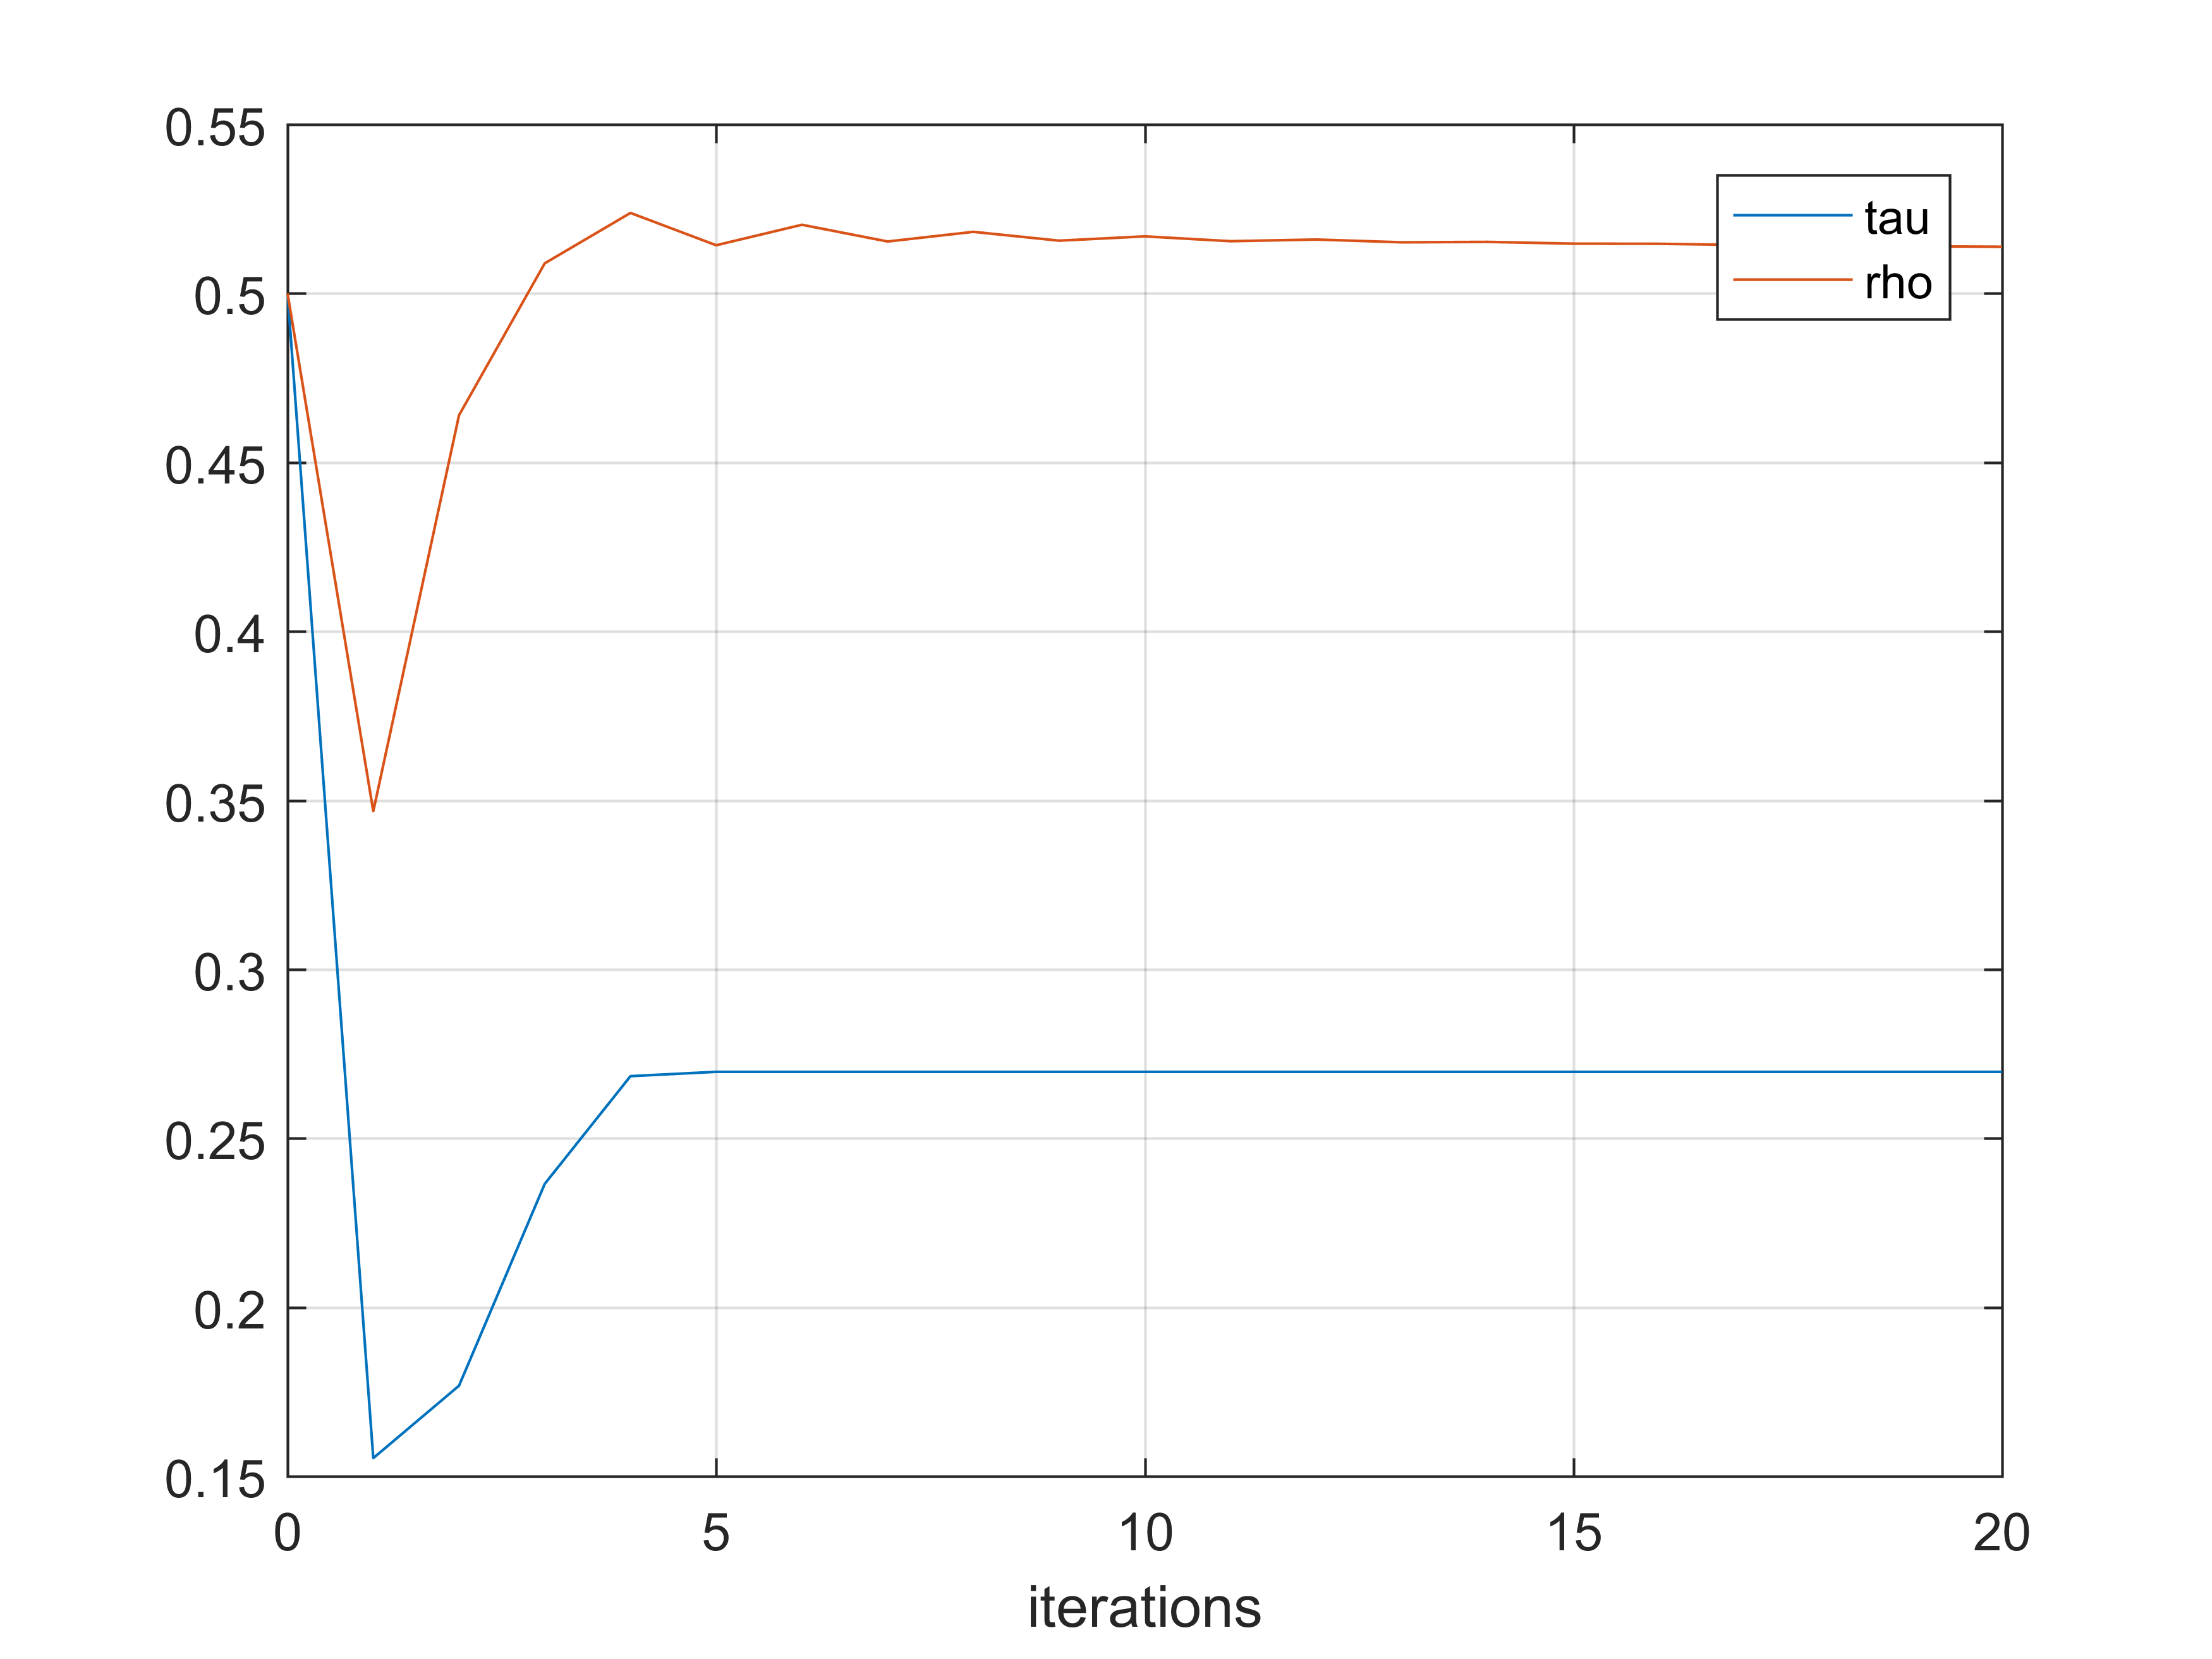
\includegraphics[width=9cm,keepaspectratio]{tau and rho.png}}
\caption{ Time factor and power factor under optimal relay user ($\alpha ^{\ast }=0.31$).}
\label{fig}
\end{figure}

\begin{figure}[htbp]
\centerline{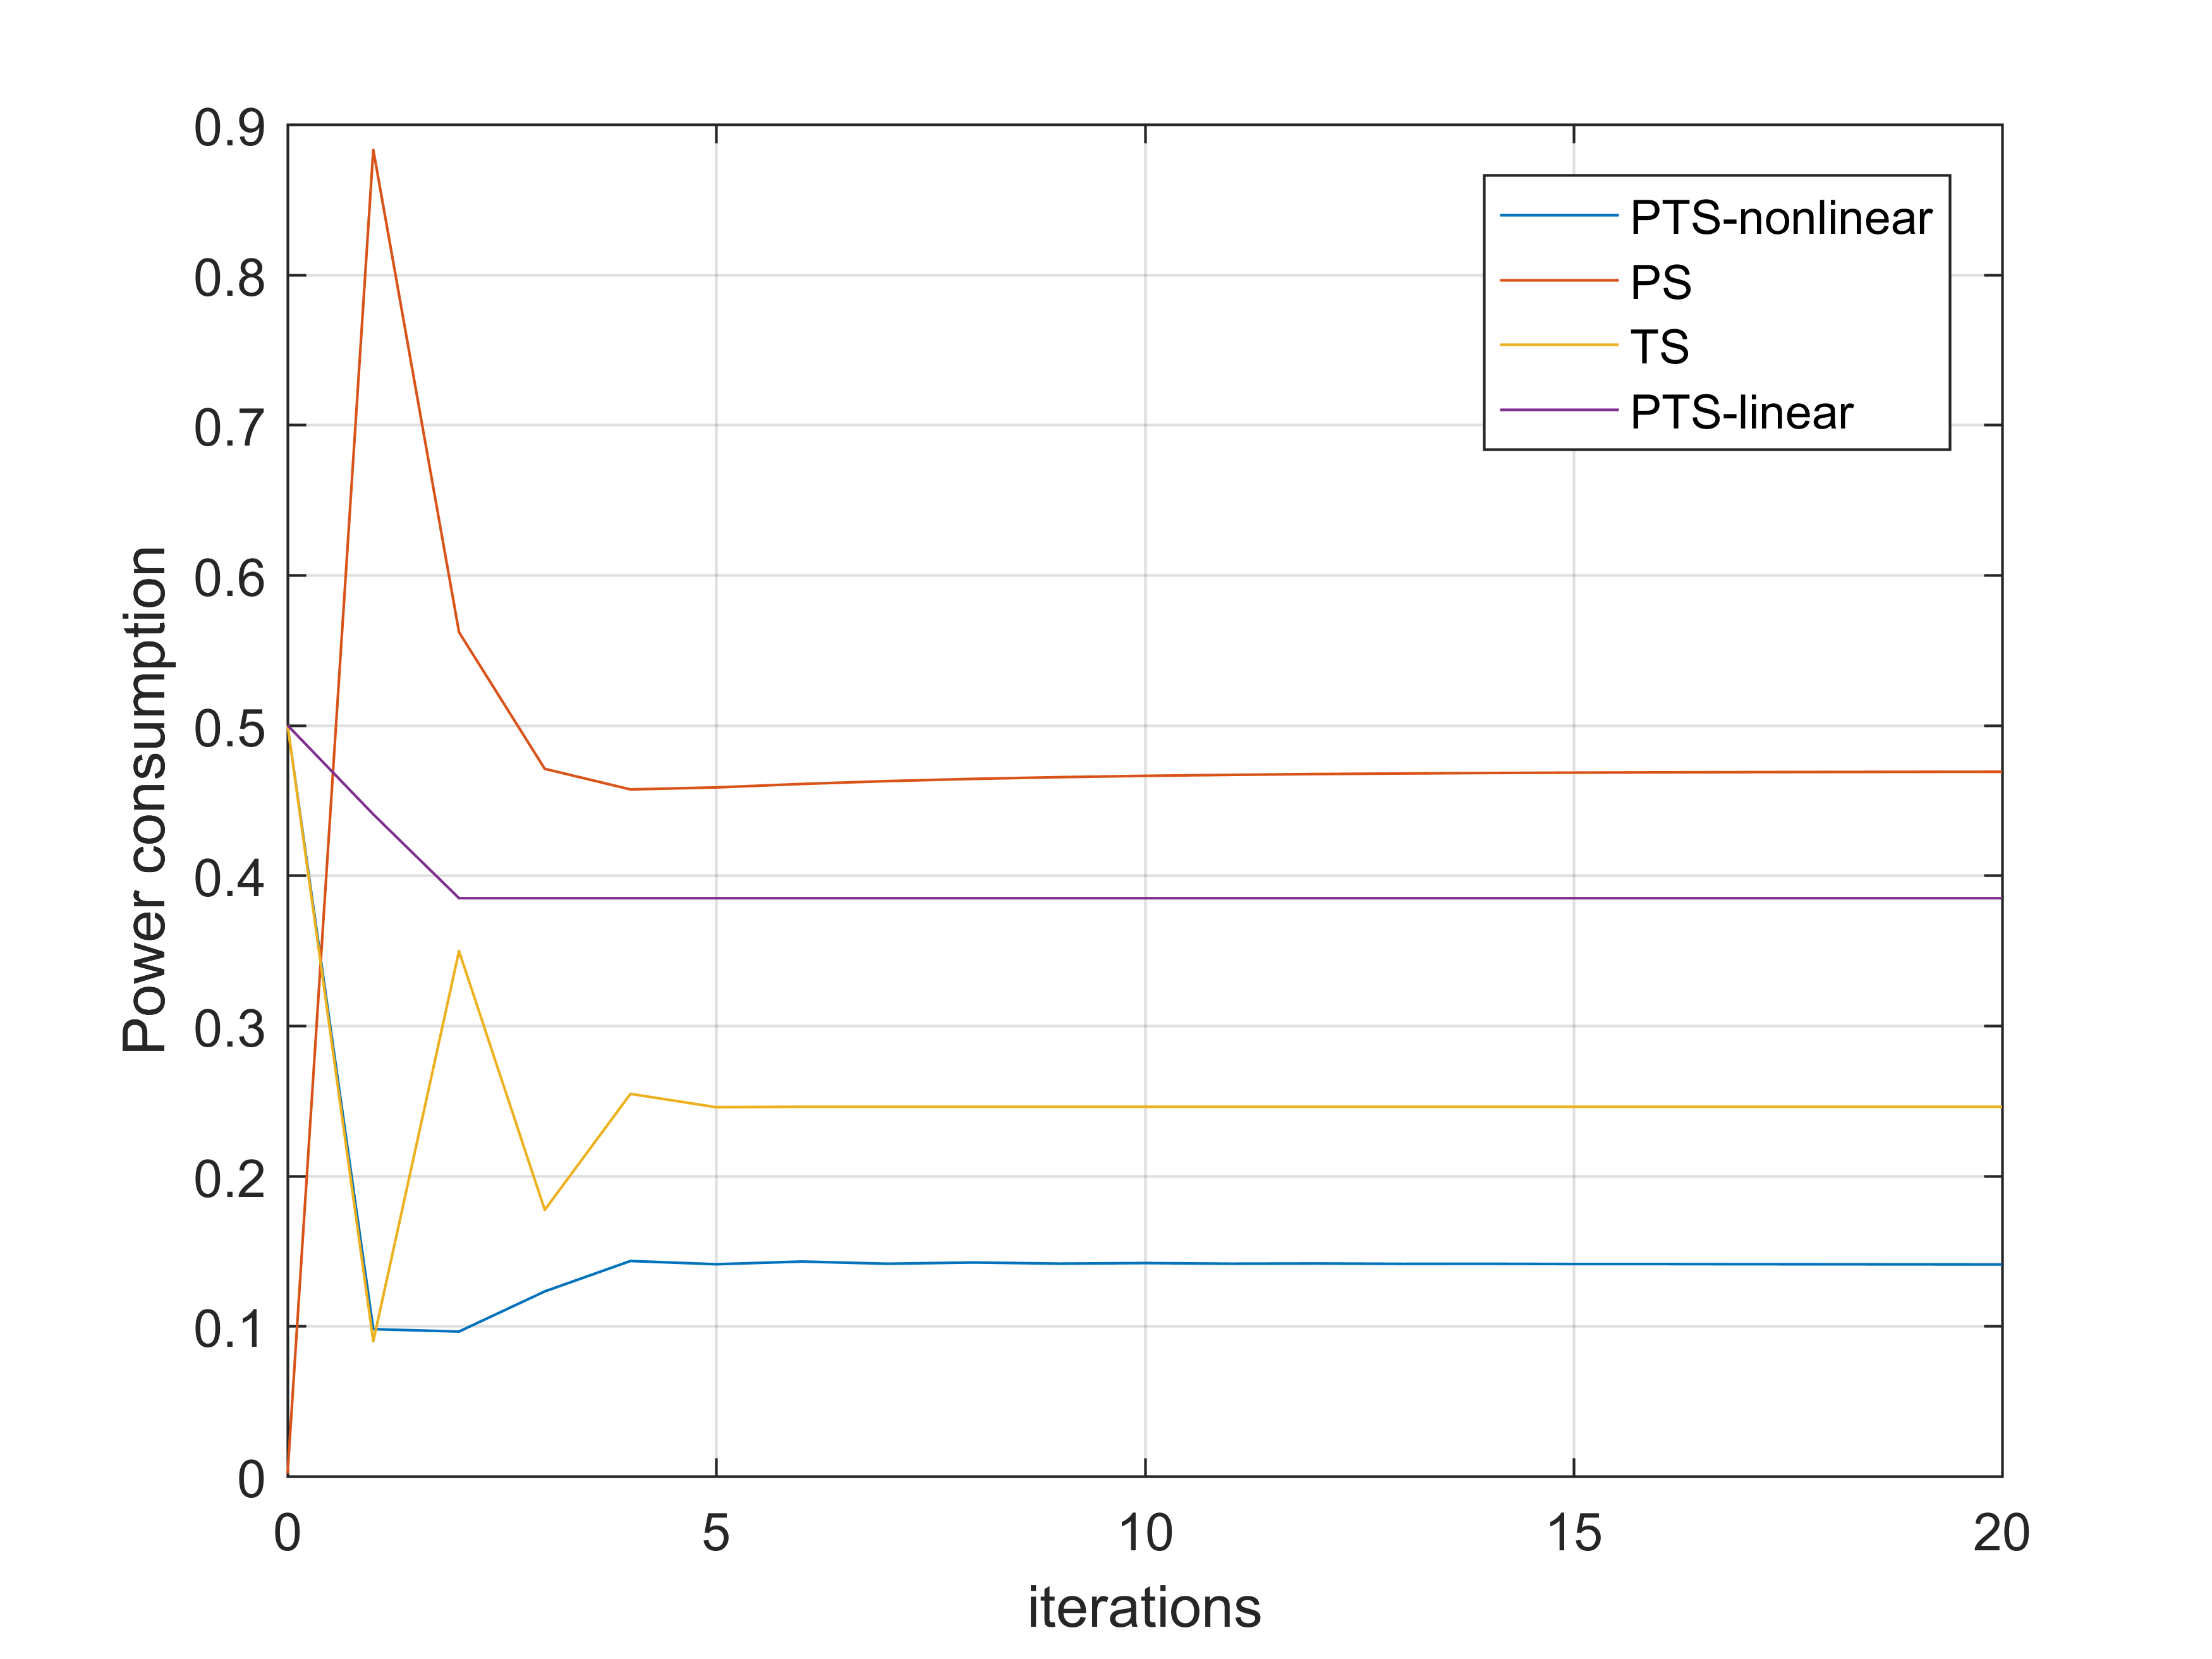
\includegraphics[width=9cm,keepaspectratio]{PTS,PS,TS,PTS(linear).png}}
\caption{ Base station energy consumption under different EH architectures.}
\label{fig}
\end{figure}

\begin{figure}[htbp]
\centerline{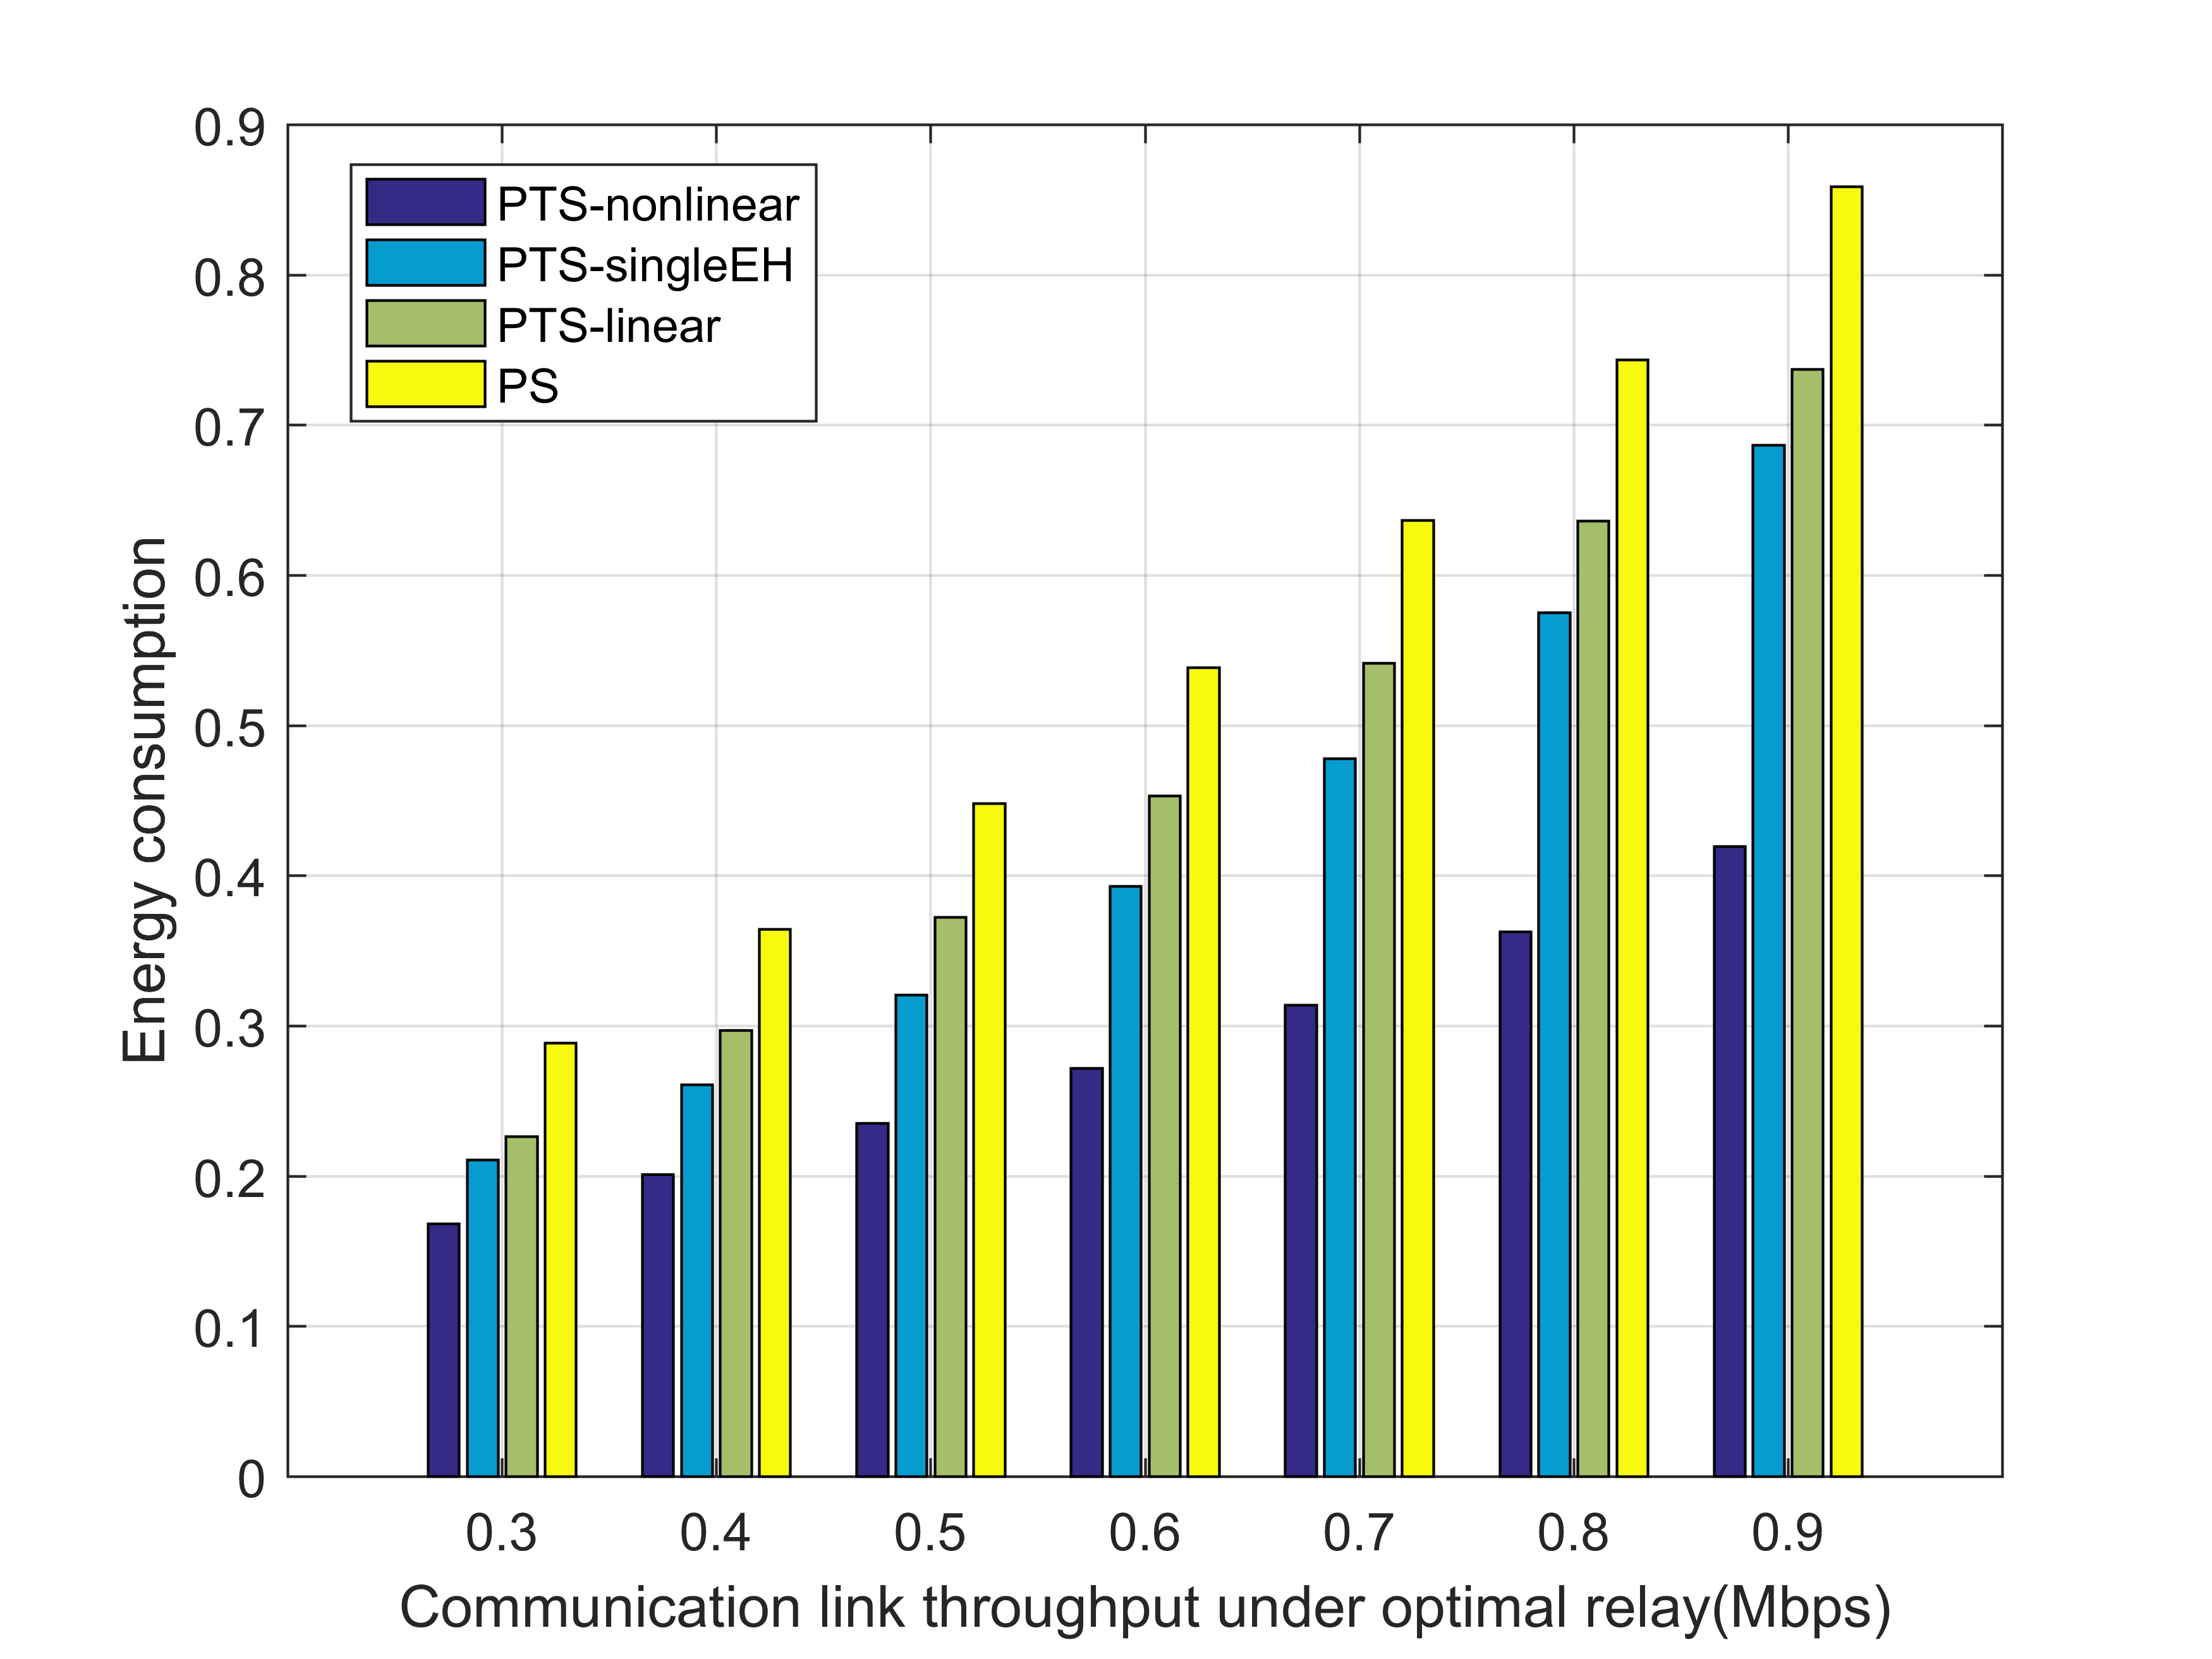
\includegraphics[width=9cm,keepaspectratio]{throughput.png}}
\caption{ The impact of throughput on base station energy consumption under different energy harvesting models.}
\label{fig}
\end{figure}

Figure 4 shows that the linear model and the nonlinear model are very different in the energy received from the RF signal emitted by the base station. The most intuitive is that the linear model will increase with the increase of the input RF power, but there is no maximum threshold. This is because only the conversion efficiency $\eta$ is fitted in the linear model, and there is no constraint of other conditions. However, in the nonlinear EH model, due to the existence of electronic devices.The nonlinear characteristics are also revealed, which can be approximated as s-curves. The maximum threshold is the parameter when the circuit is saturated. Obviously, increasing the number of EH circuits will increase this threshold, but this will also affect the conversion efficiency of RF-DC under different models, as shown in Figure 5.

Figure 5 first intuitively reflects the difference in conversion efficiency between linear models and nonlinear models. The linear EH model is a constant straight line, because its conversion efficiency is a fixed value given by the actual situation after consulting the relevant literature. In the nonlinear EH model, the conversion efficiency will be affected by the circuit parameters and the input RF power, but the trend is that the conversion efficiency increases first and then decreases with the increase of the input RF power. This is because when the input RF power is small, the EH circuit does not reach saturation, but when it continues to increase to more than the threshold value received by the EH circuit, it will cause a waste of input RF power, and the corresponding conversion efficiency will be reduced.
After increasing the number of EH circuits to two, the RF power required to saturate the EH circuit will increase accordingly, therefore, the RF power required to achieve the maximum conversion efficiency of the multi-EH circuit is greater than that of the single EH circuit.
However, the multi-EH circuit also has the disadvantage of increasing the circuit loss, so the maximum conversion efficiency is lower than that of the single EH circuit.


Figure 6 shows that there are four relay users between the base station and the target user who can carry out auxiliary communication. Considering that the location of each relay is different and the channel state information is also different, after the power minimization optimization, it can be determined that RU1 is selected as the relay and the base station energy consumption is the smallest. Figure 7 is the optimal relay RU1 parameter optimization iteration process, where $\alpha ^{\ast }=0.31 , \tau^{\ast }=0.27 , \rho^{\ast }=0.52$. In the first iteration, both $\rho$ and $\tau$ decrease numerically, which is due to the decomposition of the main optimization problem. After the initial value is given, it can be found from the figure 2 that the same input RF power, when $\rho$ decreases, the harvested energy will increase, resulting in a decrease in the time factor $\tau$. However, due to the need to ensure the communication rate, it shows an upward trend in subsequent iterations. 

Figure 8 is a comparative simulation of three different energy harvesting strategies based on power division, time division and hybrid PTS at the relay node. It can be clearly seen that under the same channel state information, the use of PTS will reduce the energy consumption of the base station. This is because it combines the advantages of PS and TS to transmit energy and information simultaneously in the same time period, and then the collected energy is fully used for communication between the relay user and the target user, which not only prolongs the life of the relay node, but also ensures the communication quality of the system.

Figure 9 shows the impact of throughput on base station energy consumption under different energy harvesting models in SWIPT system. It can be seen that the energy consumption of the base station increases with the increase of throughput, and the nonlinear PTS energy harvesting model under the multi-EH circuit used in this paper has a significant effect on reducing energy consumption. This is because the nonlinear SWIPT itself has a high conversion efficiency under a certain range of input RF power, and the multi-EH circuit also makes up for the problem of low output RF power threshold. 

\section{Conclusion}

In this paper, we establish a joint optimization model of nonlinear SWIPT relay cooperative communication system under nonlinear multi-EH circuit architecture.
By jointly optimizing power splitting ratio, time splitting ratio, beamforming vector and EH circuit architecture, the goal of minimizing base station energy consumption is achieved.
This paper uses the PTS hybrid EH model and multiple EH circuits to participate in RF-EH, which significantly reduces the energy consumption of the base station and improves the energy conversion efficiency. 
In the inner optimization problem, the non-convex to convex transformation is completed by solving the inverse function of the output RF power and other mathematical methods, and then replacing the output with the input RF power. Then the coupling between variables is eliminated by alternating iterative algorithm.
The advantage of the nonlinear EH model over the linear model is that the RF-EH conversion efficiency is higher than the linear model in a certain input RF power range. The advantage of multi-EH circuit over single EH circuit is that it avoids the problem of constant output caused by high input RF power. Compared with PS and TS models, the advantage of PTS model is that it not only ensures the quality of service of communication, but also does not lead to the problem of short life of relay nodes caused by insufficient energy collected, and also reduces the energy consumption of base stations to a certain extent.
By comparing the simulation results, the effectiveness of the hybrid model used in this paper in reducing the energy consumption of the base station is verified.


\begin{thebibliography}{00}
\bibitem{b1} G. Ma, J. Xu, Y. Zeng and M. R. V. Moghadam, "A Generic Receiver Architecture for MIMO Wireless Power Transfer With Nonlinear Energy Harvesting," in IEEE Signal Processing Letters, vol. 26, no. 2, pp. 312-316, Feb. 2019.
\bibitem{b2} R. Morsi, V. Jamali, A. Hagelauer, D. W. K. Ng and R. Schober, "Conditional Capacity and Transmit Signal Design for SWIPT Systems With Multiple Nonlinear Energy Harvesting Receivers," in IEEE Transactions on Communications, vol. 68, no. 1, pp. 582-601, Jan. 2020.
\bibitem{b3} H. Yang, Y. Ye, X. Chu and M. Dong, "Resource and Power Allocation in SWIPT-Enabled Device-to-Device Communications Based on a Nonlinear Energy Harvesting Model," in IEEE Internet of Things Journal, vol. 7, no. 11, pp. 10813-10825, Nov. 2020.
\bibitem{b4} S. Xu, X. Song, L. Xia, J. Cao, H. Qi and Z. Xie, "Optimal Power Allocation for Non-Linear EH Cooperative Network with Multiple Eavesdroppers," IECON 2020 The 46th Annual Conference of the IEEE Industrial Electronics Society, Singapore, 2020, pp. 3913-3917.
\bibitem{b5} P. V. Tuan and I. Koo, "Optimizing Efficient Energy Transmission on a SWIPT Interference Channel Under Linear/Nonlinear EH Models," in IEEE Systems Journal, vol. 14, no. 1, pp. 457-468, March 2020.
\bibitem{b6} Liu Z ,  Zhao S ,  Yuan Y , et al. Game-based approach of fair resource allocation in wireless powered cooperative cognitive radio networks[J]. AEU: Archiv fur Elektronik und Ubertragungstechnik: Electronic and Communication, 2021(134-):134.
\bibitem{b7} G. S. Sahoo and A. Ghosh, "Performance Analysis for Hybrid Beamforming Algorithm in 5G MIMO Wireless Communication System," 2022 IEEE Microwaves, Antennas, and Propagation Conference (MAPCON), Bangalore, India, 2022, pp. 592-596.
\bibitem{b8} R. Jiang, K. Xiong, P. Fan, Y. Zhang and Z. Zhong, "Power Minimization in SWIPT Networks With Coexisting Power-Splitting and Time-Switching Users Under Nonlinear EH Model," in IEEE Internet of Things Journal, vol. 6, no. 5, pp. 8853-8869, Oct. 2019.
\bibitem{b9} S. A. A. Kazmi and S. Coleri, "Optimization of Full-Duplex Relaying System With Non-Linear Energy Harvester," in IEEE Access, vol. 8, pp. 201566-201576, 2020.
\bibitem{b10} R. Jiang, K. Xiong, P. Fan, L. Zhou and Z. Zhong, "Outage Probability and Throughput of Multirelay SWIPT-WPCN Networks With Nonlinear EH Model and Imperfect CSI," in IEEE Systems Journal, vol. 14, no. 1, pp. 1206-1217, March 2020.
\bibitem{b11} P. Nezhadmohammad, M. Abedi, M. J. Emadi and R. Wichman, "SWIPT-Enabled Multiple Access Channel: Effects of Decoding Cost and Non-Linear EH Model," in IEEE Transactions on Communications, vol. 70, no. 1, pp. 306-316, Jan. 2022.
\bibitem{b12} T. M. Hoang, A. El Shafie, D. B. da Costa, T. Q. Duong, H. D. Tuan and A. Marshall, "Security and Energy Harvesting for MIMO-OFDM Networks," in IEEE Transactions on Communications, vol. 68, no. 4, pp. 2593-2606, April 2020.
\bibitem{b13} Y. Lu, K. Xiong, P. Fan, Z. Ding, Z. Zhong and K. B. Letaief, "Secrecy Energy Efficiency in Multi-Antenna SWIPT Networks With Dual-Layer PS Receivers," in IEEE Transactions on Wireless Communications, vol. 19, no. 6, pp. 4290-4306, June 2020.
\bibitem{b14} L. Li, R. Cai, H. Jiang and X. Su, "Rate-Energy Tradeoff for SWIPT Systems with Multi-User Interference Channels under Non-Linear Energy Harvesting Model," 2019 IEEE 89th Vehicular Technology Conference (VTC2019-Spring), Kuala Lumpur, Malaysia, 2019, pp. 1-6.
\bibitem{b15} Y. Lu, K. Xiong, P. Fan, Z. Ding, Z. Zhong and K. B. Letaief, "Global Energy Efficiency in Secure MISO SWIPT Systems With Non-Linear Power-Splitting EH Model," in IEEE Journal on Selected Areas in Communications, vol. 37, no. 1, pp. 216-232, Jan. 2019.
\bibitem{b16} Y. Lu, K. Xiong, J. Liu, D. Wang, P. Fan and Z. Zhong, "Secrecy Energy Efficiency in SWIPT Networks with Two-Layer Power-Splitting Receiver," 2018 IEEE Globecom Workshops (GC Wkshps), Abu Dhabi, United Arab Emirates, 2018, pp. 1-7.
\bibitem{b17} Z. Liu, M. Zhao, K. Y. Chan, Y. Yuan and X. Guan, "Approach of Robust Resource Allocation in Cognitive Radio Network With Spectrum Leasing," in IEEE Transactions on Green Communications and Networking, vol. 4, no. 2, pp. 413-422, June 2020.
\bibitem{b18} Y. Xu, H. Xie, C. Liang and F. R. Yu, "Robust Secure Energy-Efficiency Optimization in SWIPT-Aided Heterogeneous Networks With a Nonlinear Energy-Harvesting Model," in IEEE Internet of Things Journal, vol. 8, no. 19, pp. 14908-14919, 1 Oct.1, 2021.
\bibitem{b19} V. Panse, T. K. Jain and A. Kothari, "Relay Selection in SWIPT-enabled Cooperative Networks," 2022 1st International Conference on the Paradigm Shifts in Communication, Embedded Systems, Machine Learning and Signal Processing (PCEMS), Nagpur, India, 2022, pp. 62-67.
\bibitem{b20} Y. Wang, Y. Wang, F. Zhou, Y. Wu and H. Zhou, "Resource Allocation in Wireless Powered Cognitive Radio Networks Based on a Practical Non-Linear Energy Harvesting Model," in IEEE Access, vol. 5, pp. 17618-17626, 2017.
\bibitem{b21} J. -M. Kang, C. -J. Chun, I. -M. Kim and D. I. Kim, "Dynamic Power Splitting for SWIPT With Nonlinear Energy Harvesting in Ergodic Fading Channel," in IEEE Internet of Things Journal, vol. 7, no. 6, pp. 5648-5665, June 2020.
\bibitem{b22} J. -M. Kang, I. -M. Kim and D. I. Kim, "Joint Tx Power Allocation and Rx Power Splitting for SWIPT System With Multiple Nonlinear Energy Harvesting Circuits," in IEEE Wireless Communications Letters, vol. 8, no. 1, pp. 53-56, Feb. 2019.
\bibitem{b23} Z. Zhu et al., "Secrecy Rate Optimization in Nonlinear Energy Harvesting Model-Based mmWave IoT Systems With SWIPT," in IEEE Systems Journal, vol. 16, no. 4, pp. 5939-5949, Dec. 2022.
\bibitem{b24} F. A. Khan, Z. A. Malik, A. A. Nasir and M. Masood, "Relay Selection amp Power Allocation for Maximizing Sum-Throughput of a Buffered Relay Network," in IEEE Communications Letters, vol. 24, no. 6, pp. 1318-1322, June 2020.
\end{thebibliography}



\end{document}
